\chapter{Methodology}
\label{chap:methodology}

This chapter captures all methods that were used in the research. It describes the collection of data through various sources, such as publicly available time series and field measurements that are recorded in this particular study. In addition, the methods to quantify dredging volumes are explained, as well as an approach for stakeholder interviews.

\section{Data collection}
In order to analyse and draw conclusions about the situation, data collection is one of the essential preliminary steps of the project. For the Río Paraná, the data were gathered from multiple sources, as described in this section. A summary is provided in Table \ref{tab:data collection summary}.

The first source of data is the Institute of Water (INA). Since collaboration between TU Delft and INA is a central aim of this study, an “our data is your data” policy was applied, under which data are openly exchanged. Through this approach, INA provided a large number of datasets to support the research. In addition, background knowledge was shared in the form of publications and reports produced by INA staff. For example, papers authored by M. Re, L. Kazimierski, and R.N. Szupiany, among others, served as comparative background studies. Furthermore, INA supplied geospatial datasets, including bathymetric surveys and a Digital Elevation Model (DEM) of the study area.

INA also directed us to a number of public sources for further hydrodynamic analysis and GIS applications. These included flow data from multiple gauging stations and publicly available bathymetric datasets. Examples are the Sistema Nacional de Información Hídrica (SNIH), point-based water level measurements from the governmental department Alerta, and water level records from the Prefectura Naval Argentina (PNA). An overview of these datasets is provided in Table \ref{tab:data collection summary}.

Finally, additional data were obtained through our own stakeholder contacts. For example, the Dutch Embassy provided a case study on nature-based solutions (NBS) for the Paraguay River, while YPF supplied soil profile data related to dry sand mining activities in the Paraná region. More information on the approach with stakeholders can be found in Section \ref{sec:stakeholder methods}.

\begin{table}[H]
    \centering
    \renewcommand{\arraystretch}{1.2} % row spacing
    \setlength{\tabcolsep}{4pt}       % column padding
    \begin{tabularx}{\textwidth}{p{3.5cm}p{8cm}p{3.5cm}}
        \toprule
        \textbf{Name} & \textbf{Description of data type} & \textbf{Source} \\
        \midrule
        Comparative studies  & Background literature on geomorphology of similar areas & INA   \\
        INA Dataviewer         & Historical observations and simulations of water level and discharge time series & INA  \\
        DEM of lower Paraná & GeoTIFF file containing a Digital Elevation Model of the study area & INA \\
        Bathymetry (GIS) & Results from field campaigns in and around study area (2011, 2015, 2018) & INA \\
        Sand extraction permits & Agreements on locations and volumes of dredged sand & INA \\
        MarineTraffic & Live AIS vessel data & MarineTraffic \\
        Prefectura Naval Argentina  & Water level measurements & Prefectura Naval Argentina   \\
        Sistema Nacional de Informacíon Hídrica & Water level, discharge, fine and course sediment concentration & SNIH \\
        AquaMonitor & Deltares tool that represents water gains and losses based on historical satellite imagery & Deltares, Github, Google Earth Engine \\
        Bathymetry (pdf) & Detailed bathymetries along Paraná river in pdf-format & Secretaría de Transporte \\
        Google Earth & Tool that gives away satellite imagery of the globe. Can be used for a chosen time period of 1984-now & Google Earth  \\
        \bottomrule
    \end{tabularx}
    \caption{Summary of data sources}
    \label{tab:data collection summary}
\end{table}

\subsection{SNIH measurement stations}
\label{sec:measurementstations}
The measurement stations from the \textit{Sistema Nacional de Informacíon Hídrica} that were used for the data collection are discussed in this section. In order to have accurate estimations of the sediment content in the lower Paraná, it is interesting to consider its origin. As discussed in Section \ref{sec:origin sediment content}, most of the sediments in the middle Paraná originate from the Bermejo river in northern Argentina. A representative measurement station for this river is found near El Colorado, Formosa province. Here, the SNIH reports long series of measurements of water elevation, discharge and sediment concentrations.

Moving downstream, the Bermejo confluences with the Paraguay river. Merely 80 kilometers further downstream, the confluence of the Paraguay and Paraná river is located, near the city of Corrientes. Here, a drastic change in fluvial discharge occurs. Therefore, a station that represents the flow in the Middle Paraná is sought. Approximately 500 kilometers downstream of the confluence, the Túnel Subfluvial station near Santa Fe has a good amount of data. See Figure \ref{fig:rio parana map} for the location of El Colorado and Paraná (near Santa Fe). 

The two main tributaries of the Paraná that later flow into the Río de la Plata are the Paraná de las Palmas, and the Paraná-Guazú. To examine the distribution of discharge and sediment concentrations over these tributaries, two stations are selected and shown in Figure \ref{fig:flow partition}. First, the Zárate station is considered on the Paraná de las Palmas. On the Paraná-Guazú, the Brazo Largo station is selected for data analysis. Table \ref{tab:stations data collection} presents the data for all stations considered. Note that every dataset contains measurements of water level, discharge, fine sediment concentration and course sediment concentration. Most of the data is measured monthly, however some information is recorded on shorter time intervals. 


\begin{figure}
    \centering
    \includegraphics[width=0.75\linewidth]{figures/ch4/Flow partition1.png}
    \caption{Measurement stations of interest on Paraná de las Palmas and Paraná-Guazú}
    \label{fig:flow partition}
\end{figure}



\begin{table}[H]
    \centering
    \renewcommand{\arraystretch}{1.2} % extra row spacing
    \setlength{\tabcolsep}{8pt}       % extra column spacing
    \begin{tabular}{lllc}
        \toprule
        \textbf{Station} & \textbf{SNIH ID} & \textbf{River} & \textbf{Data availability} \\
        \midrule
        El Colorado         & 2602 & Bermejo               & 1968--2025 \\
        Túnel Subfluvial    & 3050 & Middle Paraná         & 1983--2025 \\
        Zárate              & 4001 & Paraná de las Palmas  & 1993--2025 \\
        Brazo Largo         & 4002 & Paraná-Guazú          & 1993--2025 \\
        \bottomrule
    \end{tabular}
    \caption{Selection of SNIH measurement stations.}
    \label{tab:stations data collection}
\end{table}



\subsection{Dredging quantities}
The number of vessels involved in dredging activities on the Paraná Guazú was determined using AIS (Automatic Identification System) data. Vessel movements between dredging sites and ports were monitored through \textit{MarineTraffic}. Although historical records were not considered, the daily activity observed during the study period provides a reliable estimate of the sand extraction volumes. 

Alternatively, a collection of dredging permits is considered. To avoid adverse impacts on the hydraulic regime of the river due to dredging, companies must first obtain permits from the \textit{National Water Institute }(INA). These permits specify the locations and volumes of the proposed dredging activities. The information they provide serves as a reliable estimate of the total material being removed from the river, thereby influencing the sediment balance. Therefore, the permits were analysed for the area of interest.

Subsequently, the information gathered from AIS data and extraction permits were combined, resulting in estimates of volumes that are dredged in the study area. In addition, conversations with stakeholders were of valuable insight and supported the comparison with the results of the data collection. 

\section{Field study}
In the fourth week of the project the field work took place. The goal of the field work was to obtain data from measurements on the boat using different devices, as well as obtaining resourceful information from chosen stakeholders in the area of the field work. This data would then be filtered, analysed and used to take conclusions from our initial hypothesis's regarding the study.

The field work divided the group of six students in two, leaving one group of three on the boat with our supervisor of INA to take the required measurements, and one group of three with another colleague of INA for the interviews.

\subsection{Stakeholders}
\label{sec:stakeholder methods}
In this study, a qualitative research was conducted to explore perceptions and experiences related to the river. For this, interviews were conducted to capture insights from participants with diverse perspectives.

A qualitative approach was chosen because it allows for a detailed understanding of participants’ views and interpretations of the river. This design is particularly suited to capture the complexity of social and environmental issues, and to highlight the ways in which different stakeholders experience and assign meaning to the river.

Data were collected through semi-structured interviews, a method that combines prepared guiding questions with the flexibility to follow up on unexpected but relevant topics raised by participants. This format ensured that key themes were consistently addressed across interviews, while also allowing interviewees to elaborate on issues they considered important. In practice, a topic guide with questions per stakeholder was developed to provide structure, but the interviewer encouraged open-ended responses and probed further where clarification or depth was needed. Ten interviews were conducted. During the interview, responses were written down in key words. The questions along with these unfiltered results are given in Appendix \ref{chap:interviews}.

On Wednesday, the 24th of September, interviews were conducted with the caretaker at the local Fisher's club (Club de Pescadores Olivos), the port manager at Puerto Ibicuy, the Mayor of Ibicuy and a landowner in the area of Ibicuy. The caretaker and landowner showed multiple erosion banks around the river. On Thursday 25 September, interviews with the Municipality of Zarate, a local sand miner and a camping owner were carried out. The local sand miner showed the mining process on his vessel and in the port and the land owner showed their land. On this day, several drone images were also made. Finally, on Friday 26 September, the plant manager of the YPF dry sand mine and another person from the municipality of Zárate were interviewed. 

Most of the stakeholders do not speak English, which is why colleagues Marina and Martin from INA have translated the questions and responses for us. Most stakeholders were approached on site. The port manager and the mayor had already been contacted in advance. After each interview, permission was asked to quote and name the stakeholder in the report. All stakeholders have agreed to this and were willing to share their experiences. The following table represents the interviews in a scheduled manner. 

\begin{table}[H]
    \centering
    \renewcommand{\arraystretch}{1.2}
    \setlength{\tabcolsep}{4pt}
    \begin{tabularx}{\textwidth}{l l X c}
        \toprule
        \textbf{Date} & \textbf{Occupation} & \textbf{Location} & \textbf{Language} \\
        \midrule
        24-09-2025 & Caretaker at Fisher's club & 6RJF+C7, Ibicuy, Entre Ríos & Spanish \\
        24-09-2025 & Port manager at Puerto Ibicuy & 6RRC+VC, Ibicuy, Entre Ríos & Spanish \\
        24-09-2025 & Mayor of Ibicuy & 7R5R+4G Puerto Ibicuy, Entre Ríos & Spanish \\
        24-09-2025 & Landowner (Jorge) & 7R5R+4G Puerto Ibicuy, Entre Ríos and his private land & Spanish \\
        25-09-2025 & Municipality Zarate & GLO, Av. Rivadavia 751, B2800GLO Zárate, Provincia de Buenos Aires & Spanish \\
        25-09-2025 & Dredger & Caminera a Ibicuy, Entre Ríos & Spanish \\
        25-09-2025 & Camping owner & Ruta 45 Km 5, E2823, Entre Ríos & Spanish \\
        26-09-2025 & Plant manager YPF & 7XPC+72 Parnacito, Entre Ríos & English \\
        26-09-2025 & Municipality of Zarate & Leandro M. Alem 780, Zárate & Spanish \\
        \bottomrule
    \end{tabularx}
    \caption{Stakeholder overview}
    \label{tab:stakeholders}
\end{table}

\subsection{Measurement variables and equipment}
In this subsection the location and type of measurements will be explained. The goal of the field work was to obtain data from critical sections in the study area. These locations were selected in such a way that they were as useful as possible for establishing the sediment balance. Two important locations in the study area are the confluence from the Ibicuy and Paraná Guazú, and that of the Paraná Guazú and Talabera. In these sections, sediment samples and flow measurements were recorded.
Once this data was gathered, it was analysed and compared to previously obtained data to draw conclusions. 


% \begin{figure}[H]
%     \centering
%     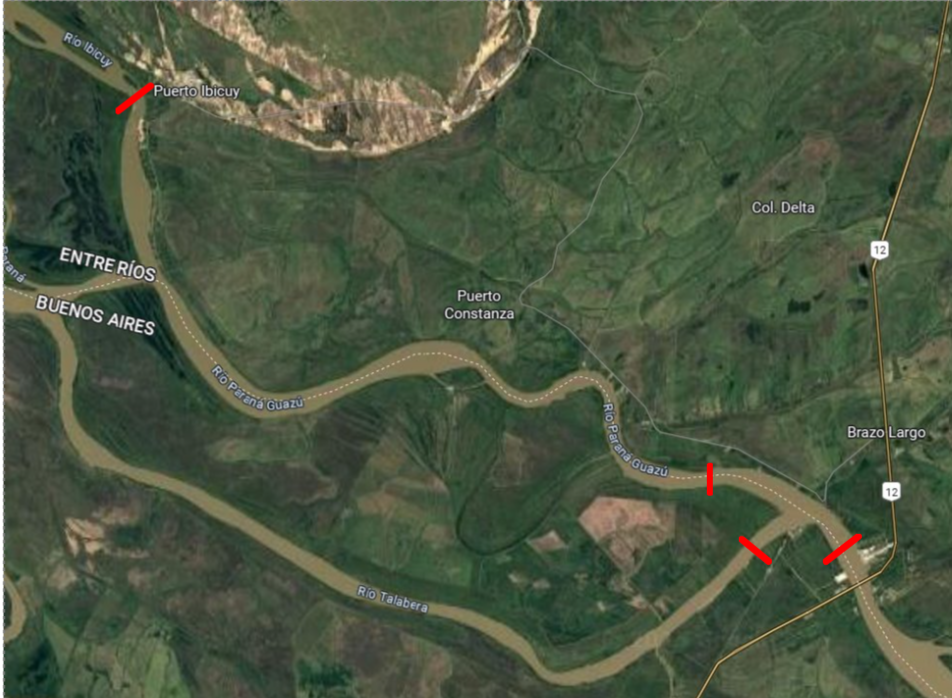
\includegraphics[width=0.5\linewidth]{figures/ch4/Critical measurement points.png}
%     \caption{Critical Cross Section Measurements}
%     \label{fig:fieldwork cross sections}
% \end{figure}

During the field trip, half of the group worked together with the INA team of employees who joined us. The team consists of one skipper who was responsible for driving the boat and one supervisor who helped us with collecting measurements. The material that was needed for the measurements was provided by INA. 

% The program of the boat days consisted of going over the indicated critical cross sections (in red on Figure 4.2) a total of 4 times, using the equipment of INA to save the necessary information of the river. 

\subsubsection{Flow velocity}
The first variable that was measured is the flow velocity profile of the river, recorded by a SonTek RiverSurveyor M9 Acoustic Doppler Current Profiler (ACDP). This device consists of two components both placed on a floating board held next to the boat while advancing. The components are a vertical acoustic echo sounder beam placed on the back end of the floating board, and a rectangle shape box containing a microprocessor that computes the data on the front end of the board, as seen in Figure \ref{fig:sontek}.

\begin{figure}[htbp]
    \centering
    \begin{subfigure}[b]{0.48\textwidth}
        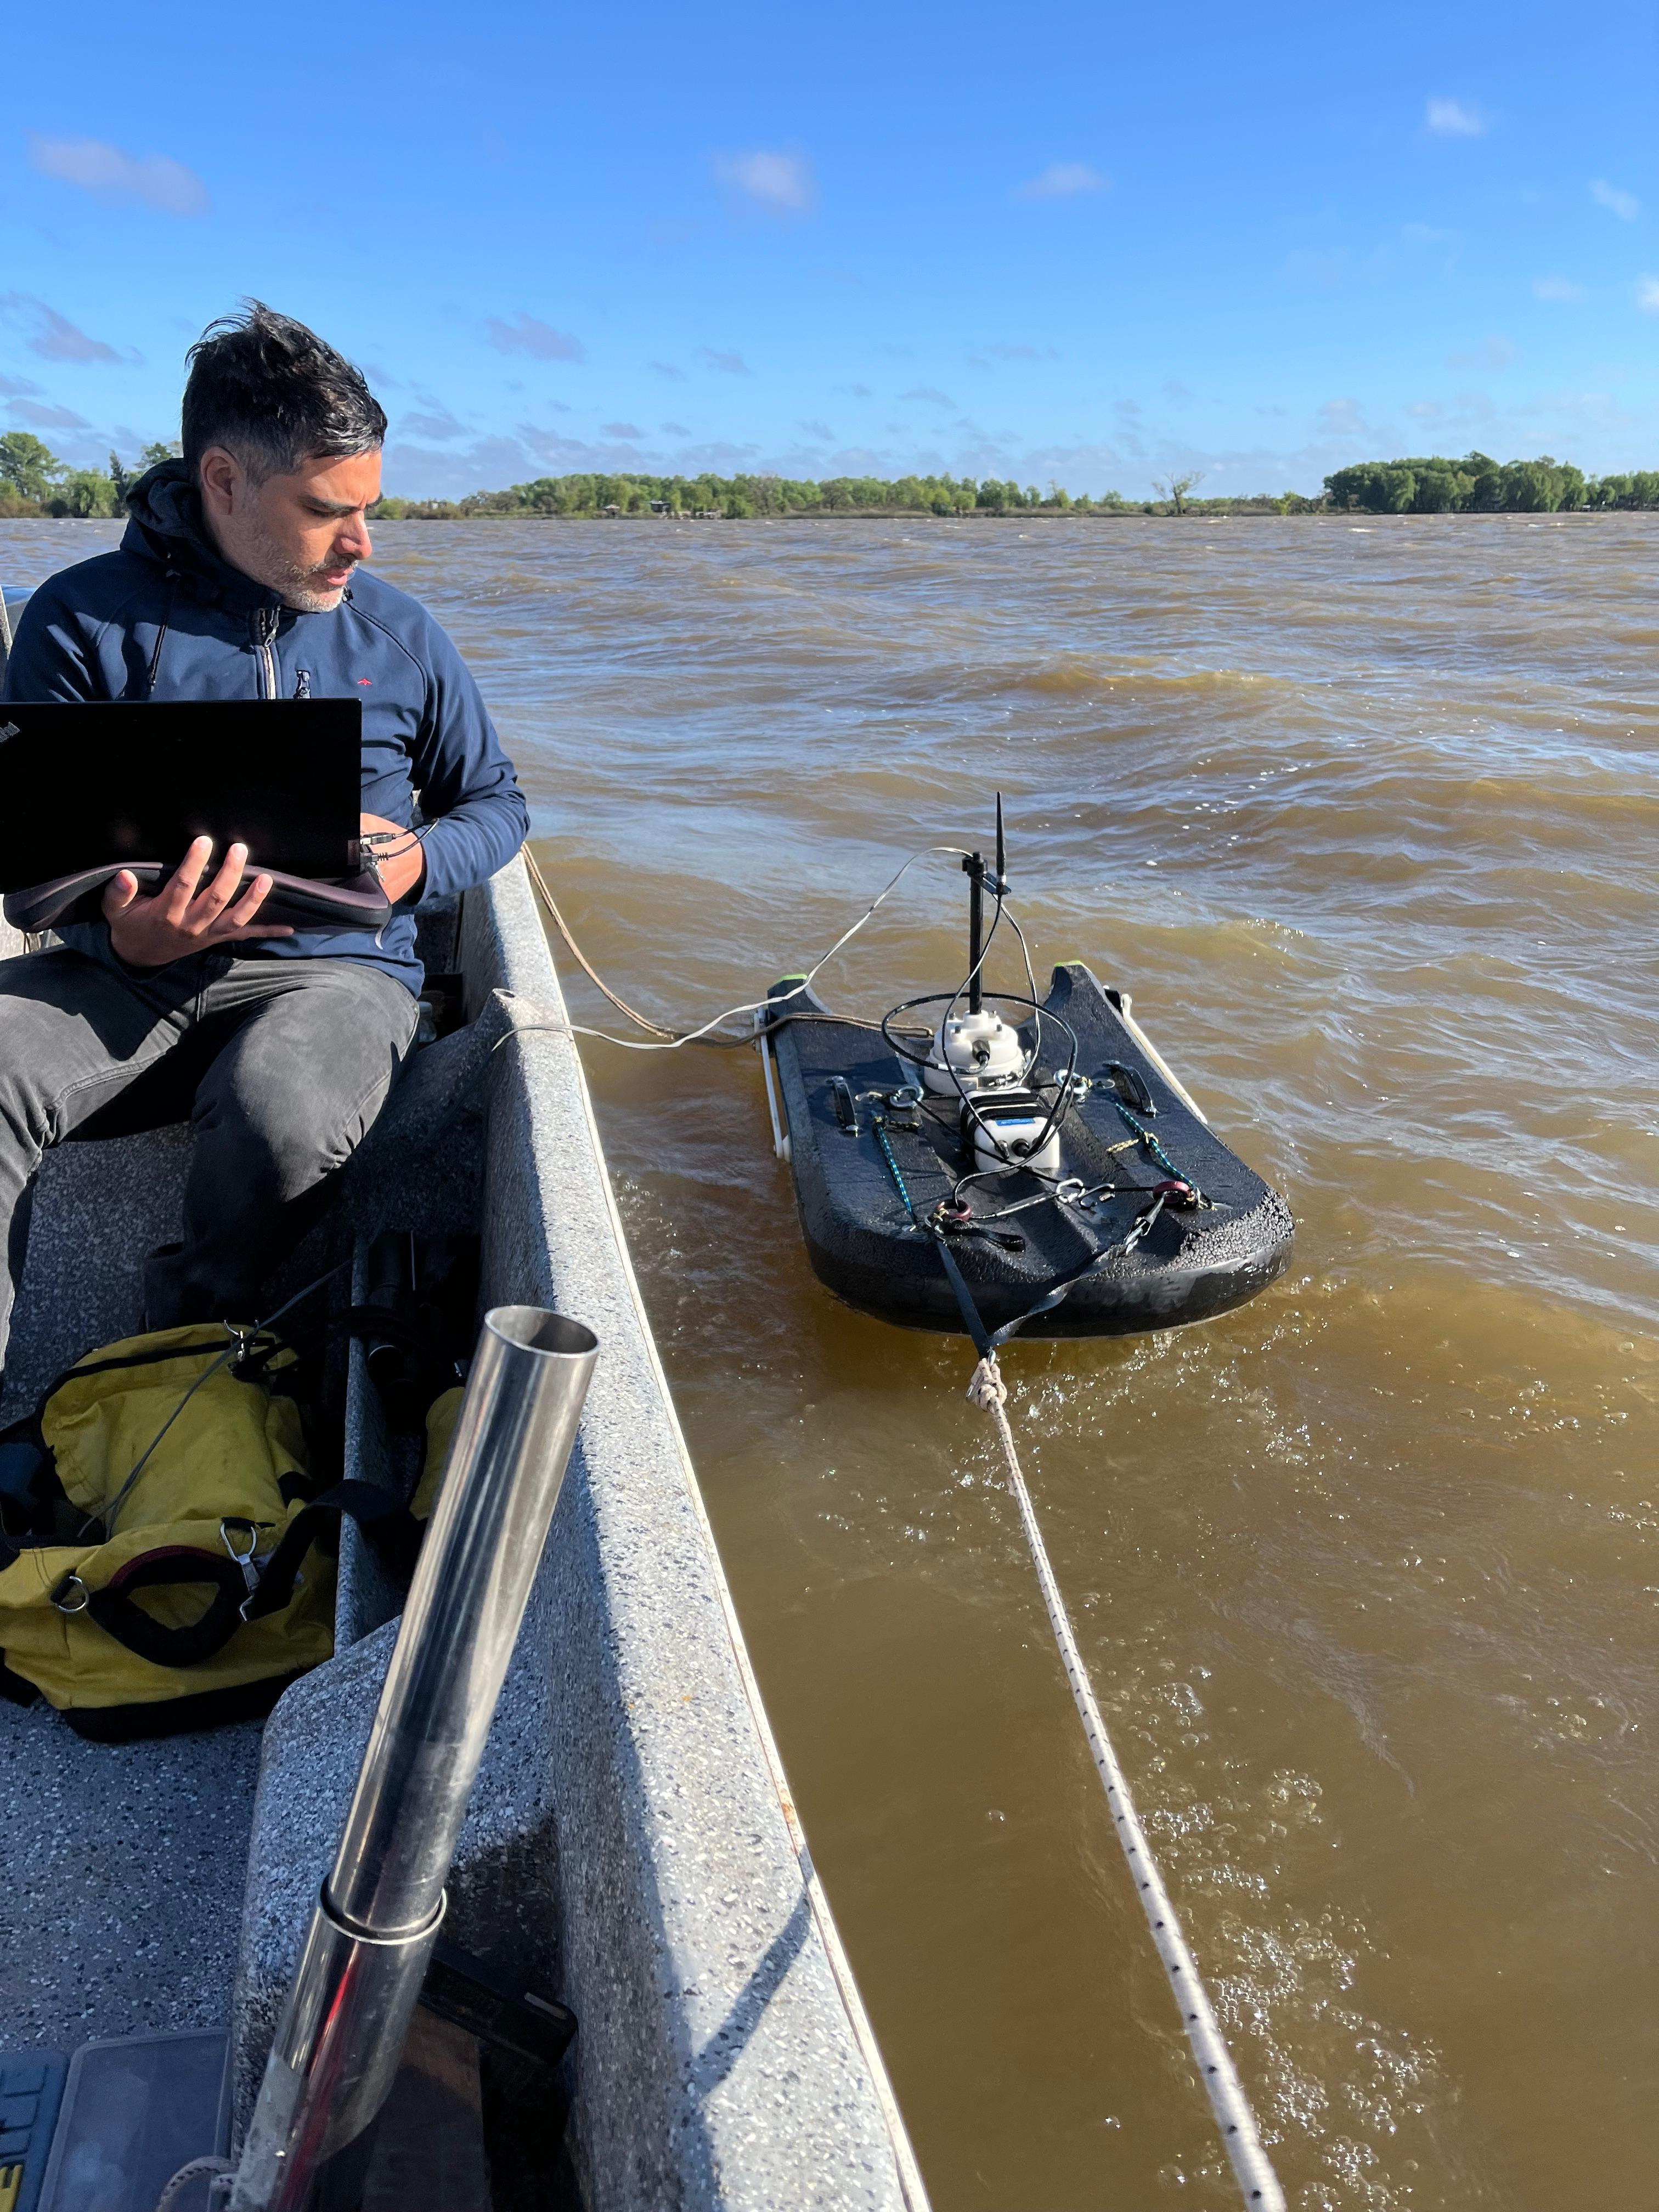
\includegraphics[width=\linewidth, height=7cm]{figures/ch4/sonteknico.jpg}
        \caption{INA supervisors helping with measurement material}
        \label{fig:sontek}
    \end{subfigure}
    \hfill
    \begin{subfigure}[b]{0.48\textwidth}
        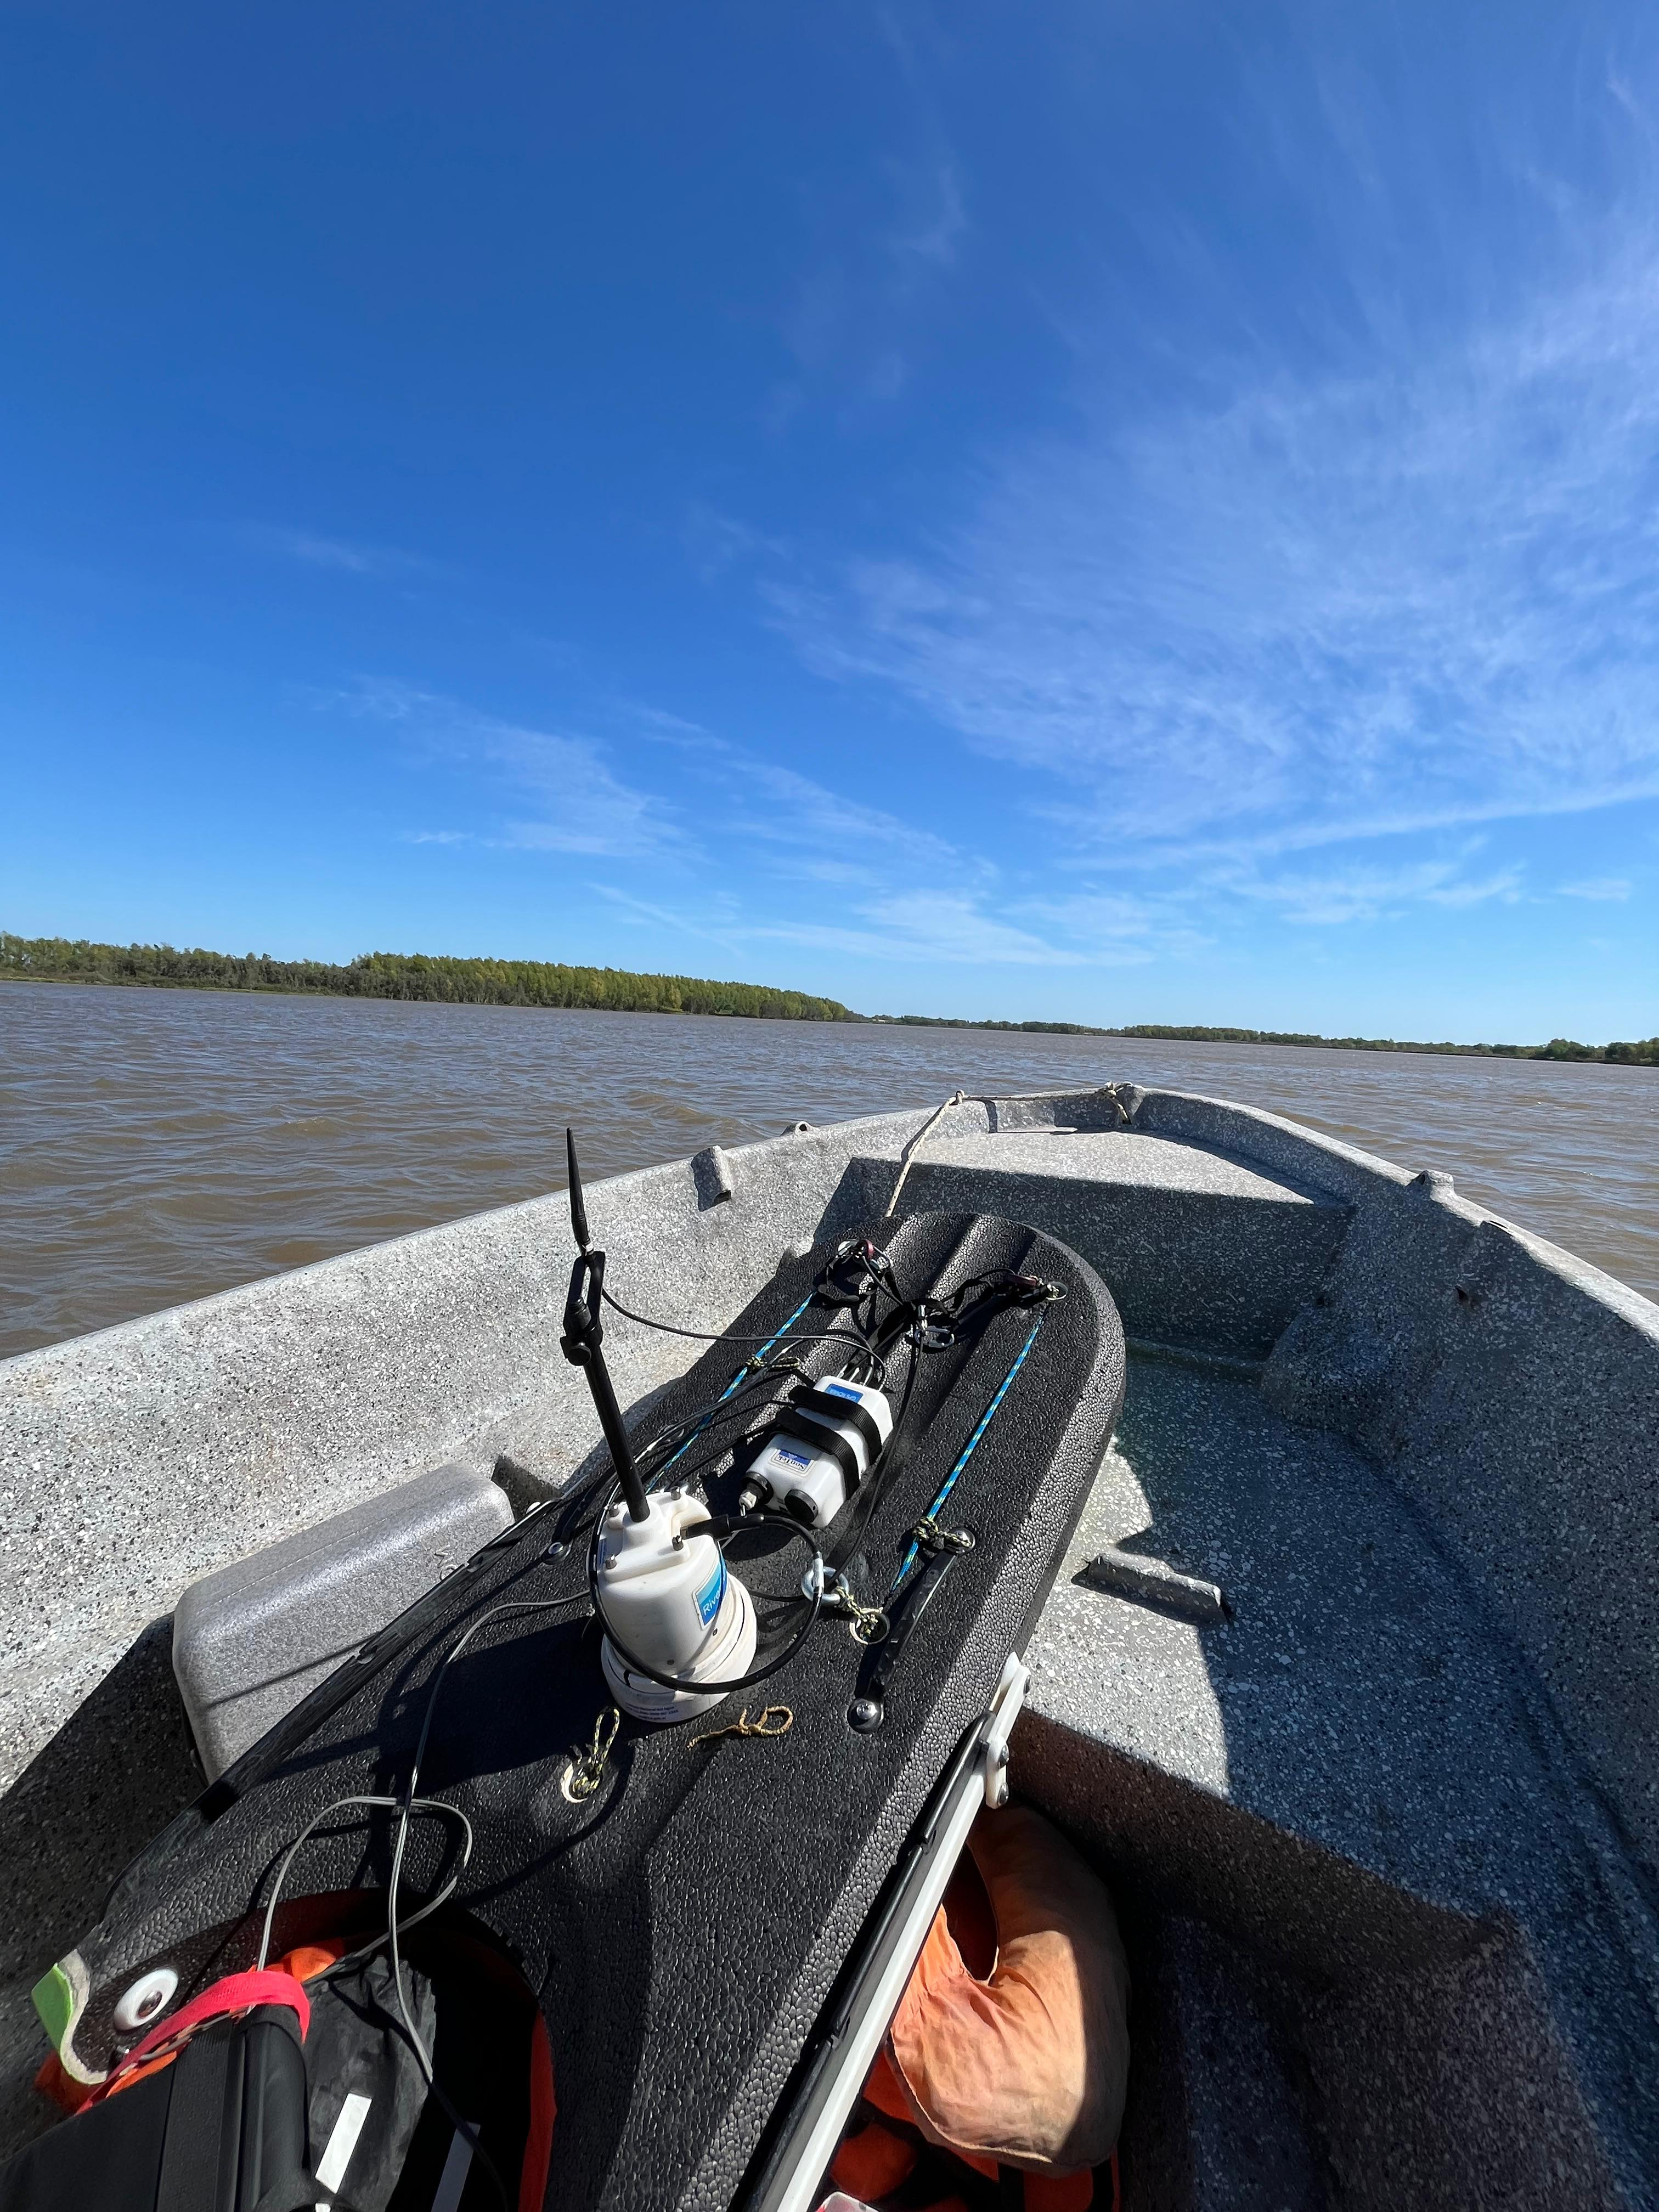
\includegraphics[width=\linewidth, height=7cm]{figures/ch4/sontek.jpg}
        \caption{SonTek M9 on the boat}
        \label{fig:sontek}
    \end{subfigure}
    \caption{SonTek M9 installed in the field}
    \label{fig:measurement}
\end{figure}

The specialty of the SonTek M9 is that it uses multiple acoustic frequencies to find a high resolution range of depths and flow velocities, while still tracking the geo-referenced position of the vessel using GNSS \autocite{advanced river discharge}. The flow velocity is the speed of the river in a certain direction. The unit is therefore  [m/s], and is expressed in the form of a vector. The significance of this data is also due to the fact that the velocity is needed to compute the discharge as well.

\subsubsection{Discharge}
Once the flow velocity \(\mathbf{v}\) is found, it can be integrated over the depth and the width of the channel (through a cross-section) which in the end yields the discharge \(Q\) of the river at a given location, with a unit of \si{\cubic\metre}/s.
\begin{equation}
    Q = \iint_A \mathbf{v} \cdot d\mathbf{A}
    \label{eq:discharge_integration}
\end{equation}

\noindent where:
\begin{itemize}
    \item \(Q\) is the discharge, expressed in cubic meters per second [m\textsuperscript{3}/s];
    \item \(\mathbf{v}\) is the flow velocity vector, expressed in meters per second [m/s];
    \item \(A\) is the cross-sectional area perpendicular to the flow, expressed in square meters [m\textsuperscript{2}];
    \item \(d\mathbf{A}\) is an infinitesimal area element.
\end{itemize}

The number of required measurements of a single cross section is defined by the variability of the measurements. That is, a minimum of two measurements exists, which is sufficient when the second discharge measurement is within 10\% of the first one. In addition, correct operation of the vessel's velocity is essential for reliable discharge results. Therefore, the boat speed should never exceed the flow velocity perpendicular to the cross section under consideration. 



% The aim of the field work was to obtain the data of flow velocity and discharge at the three critical points around the bifurcation of interest during different times, one in the morning and in the afternoon. Consequently this would indicate some changes in discharge for different times, flows, circumstances hence solidifying our data base of examples. 



\subsubsection{Suspended sediment}
Moving on, it is also in our interest to gather data on the suspended sediment concentration of the river. This is done by collecting water with the help of an APEMA BS6A peristaltic pump connected to two plastic tubes. The first tube is short and is used to insert the water into the plastic bottles on the boat. The second tube is long and is connected to a weight, which can be lowered into the river to a certain depth. At the desired depth, the fluid was pumped to the water surface and collected in the plastic bottles.

Then, the samples were sealed in order to be sent to the water quality lab in the hydraulic section on the INA site, as seen in Figure \ref{fig:suspended sediment}. These samples help to indicate the concentration of fine sediments in the channel, at different locations and elevations. The evolution of the concentrations along the study area will be studied in the Chapter \ref{chapter:data analysis}.

\begin{figure}[H]
    \centering
    % First row of subfigures
    \begin{subfigure}[b]{0.48\textwidth}
        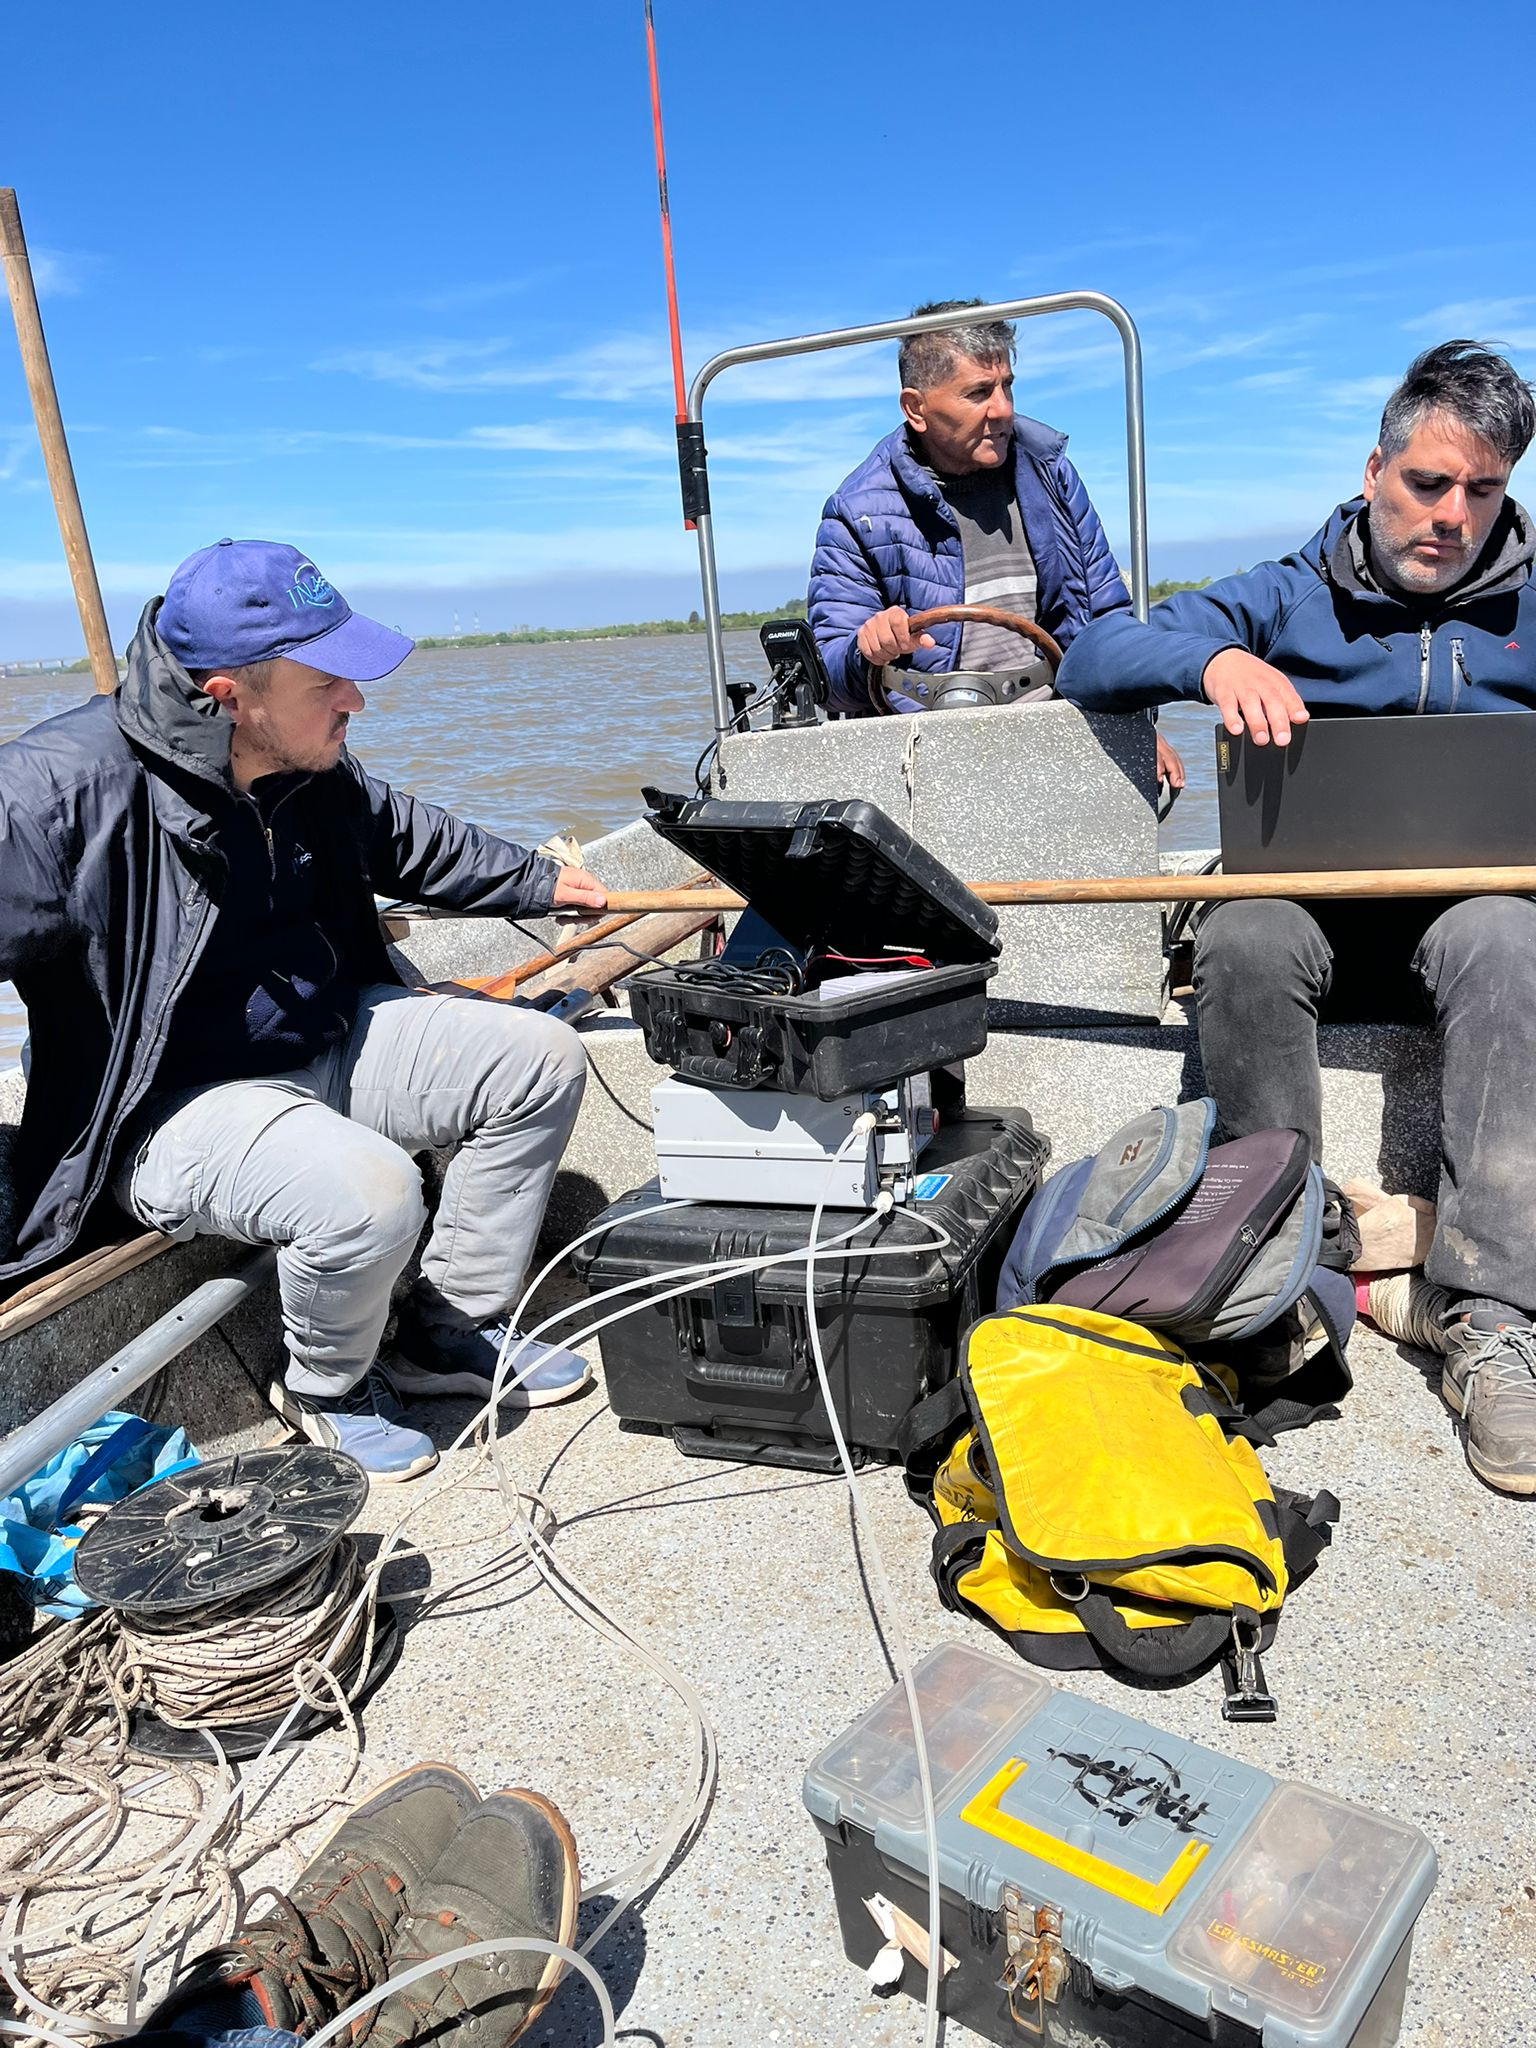
\includegraphics[width=\linewidth, height=7cm]{figures/ch4/group.jpg}
        \caption{Group picture of INA working}
        \label{fig:first}
    \end{subfigure}
    \hfill
    \begin{subfigure}[b]{0.48\textwidth}
        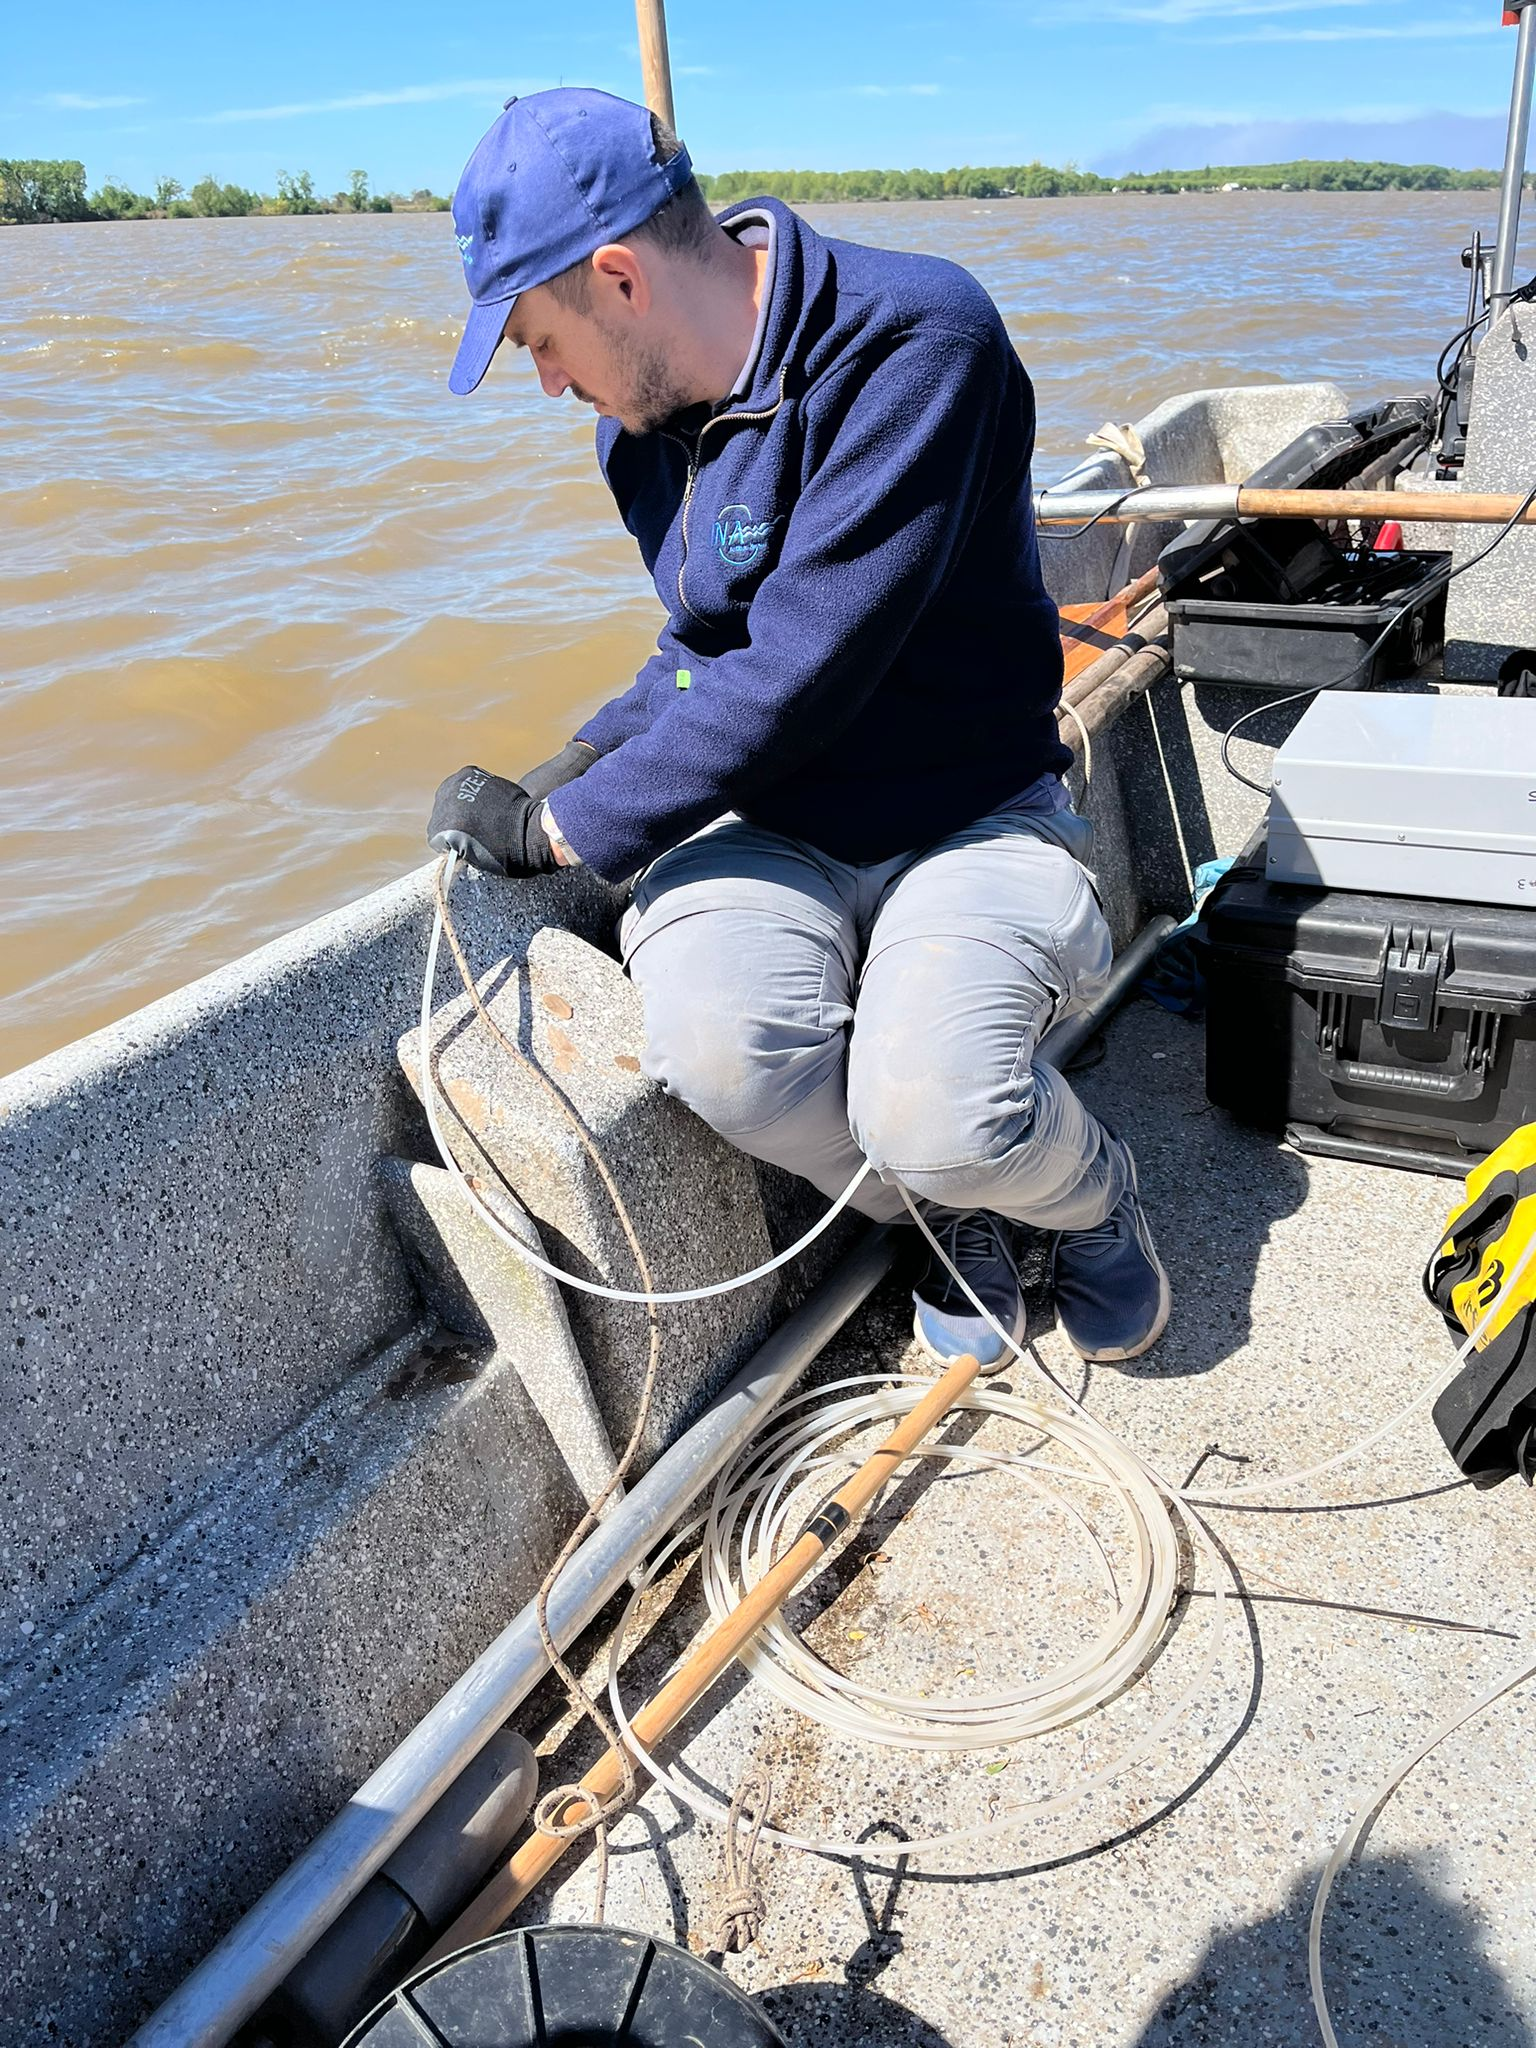
\includegraphics[width=\linewidth, height=7cm]{figures/ch4/installing.jpg}
        \caption{Installing the device}
        \label{fig:second}
    \end{subfigure}

    % Second row of subfigures (add some vertical space)
    \vspace{0.5cm}

    % Second row of subfigures
    \begin{subfigure}[b]{0.48\textwidth}
        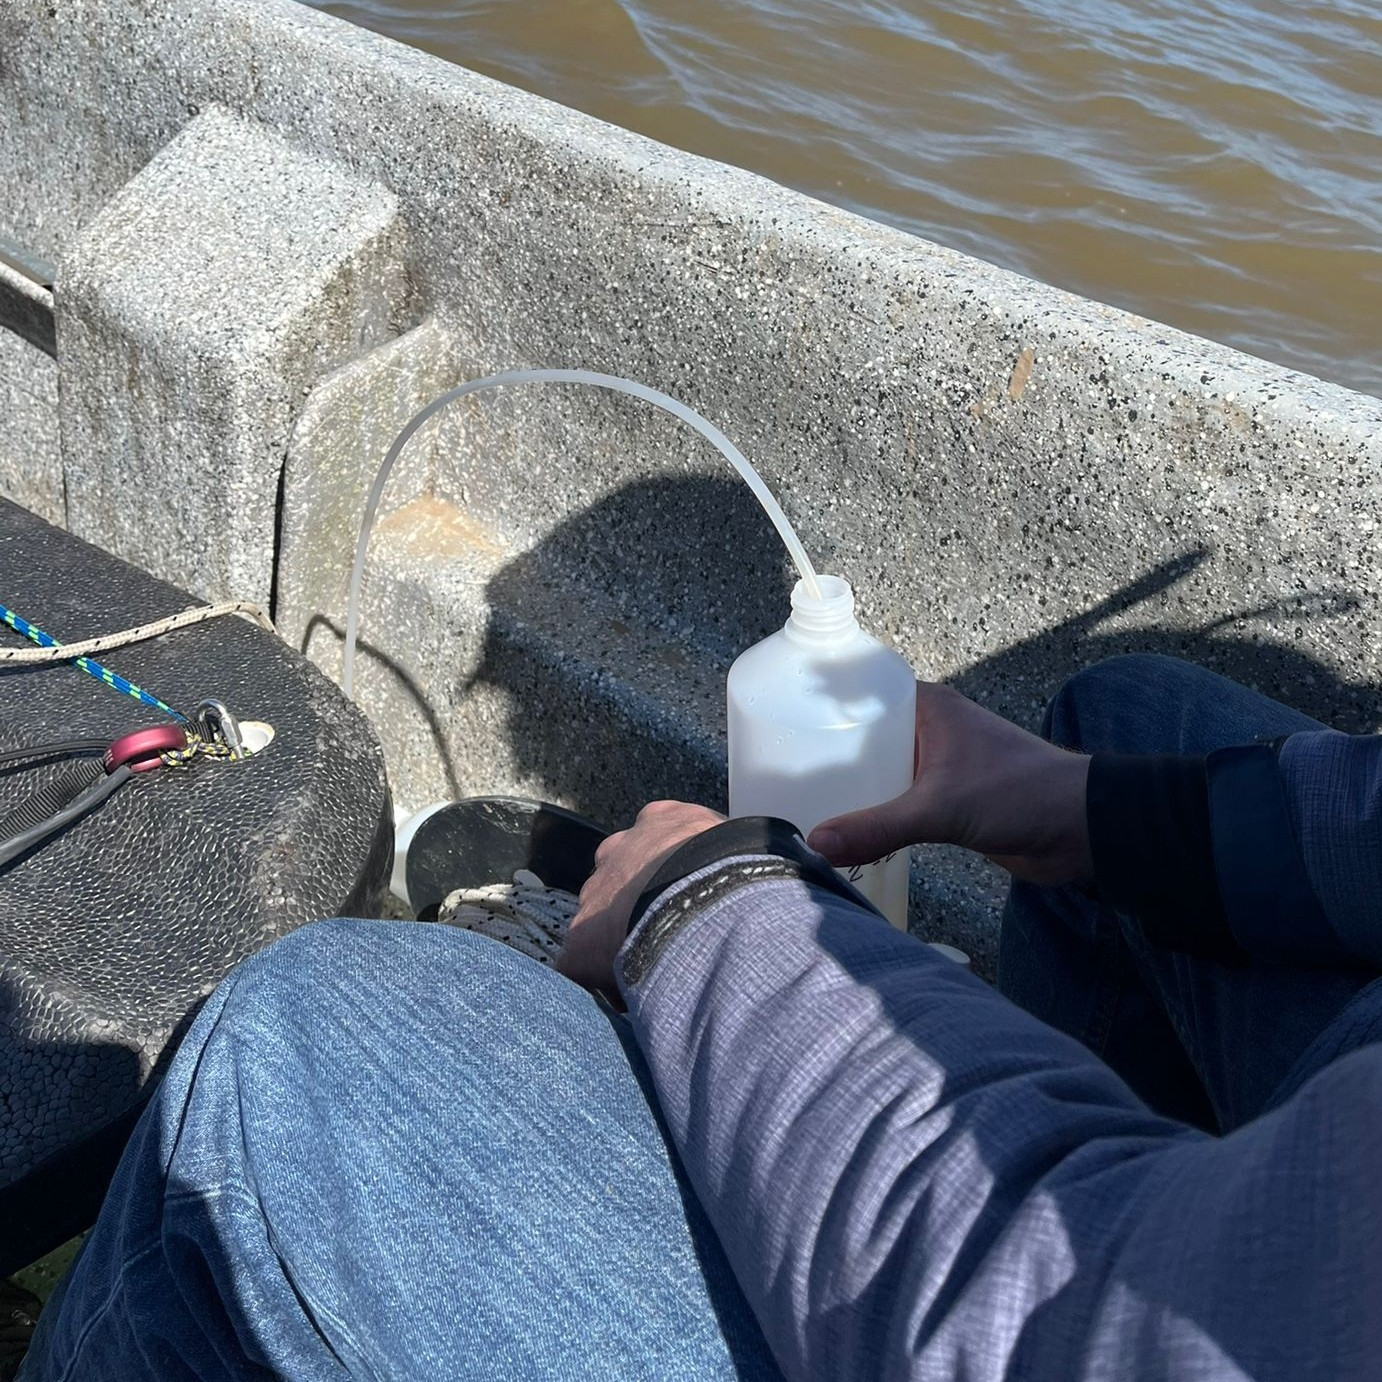
\includegraphics[width=\linewidth, height=7cm]{figures/ch4/fles.jpg}
        \caption{Bottle of water connected}
        \label{fig:third}
    \end{subfigure}
    \hfill
    \begin{subfigure}[b]{0.48\textwidth}
        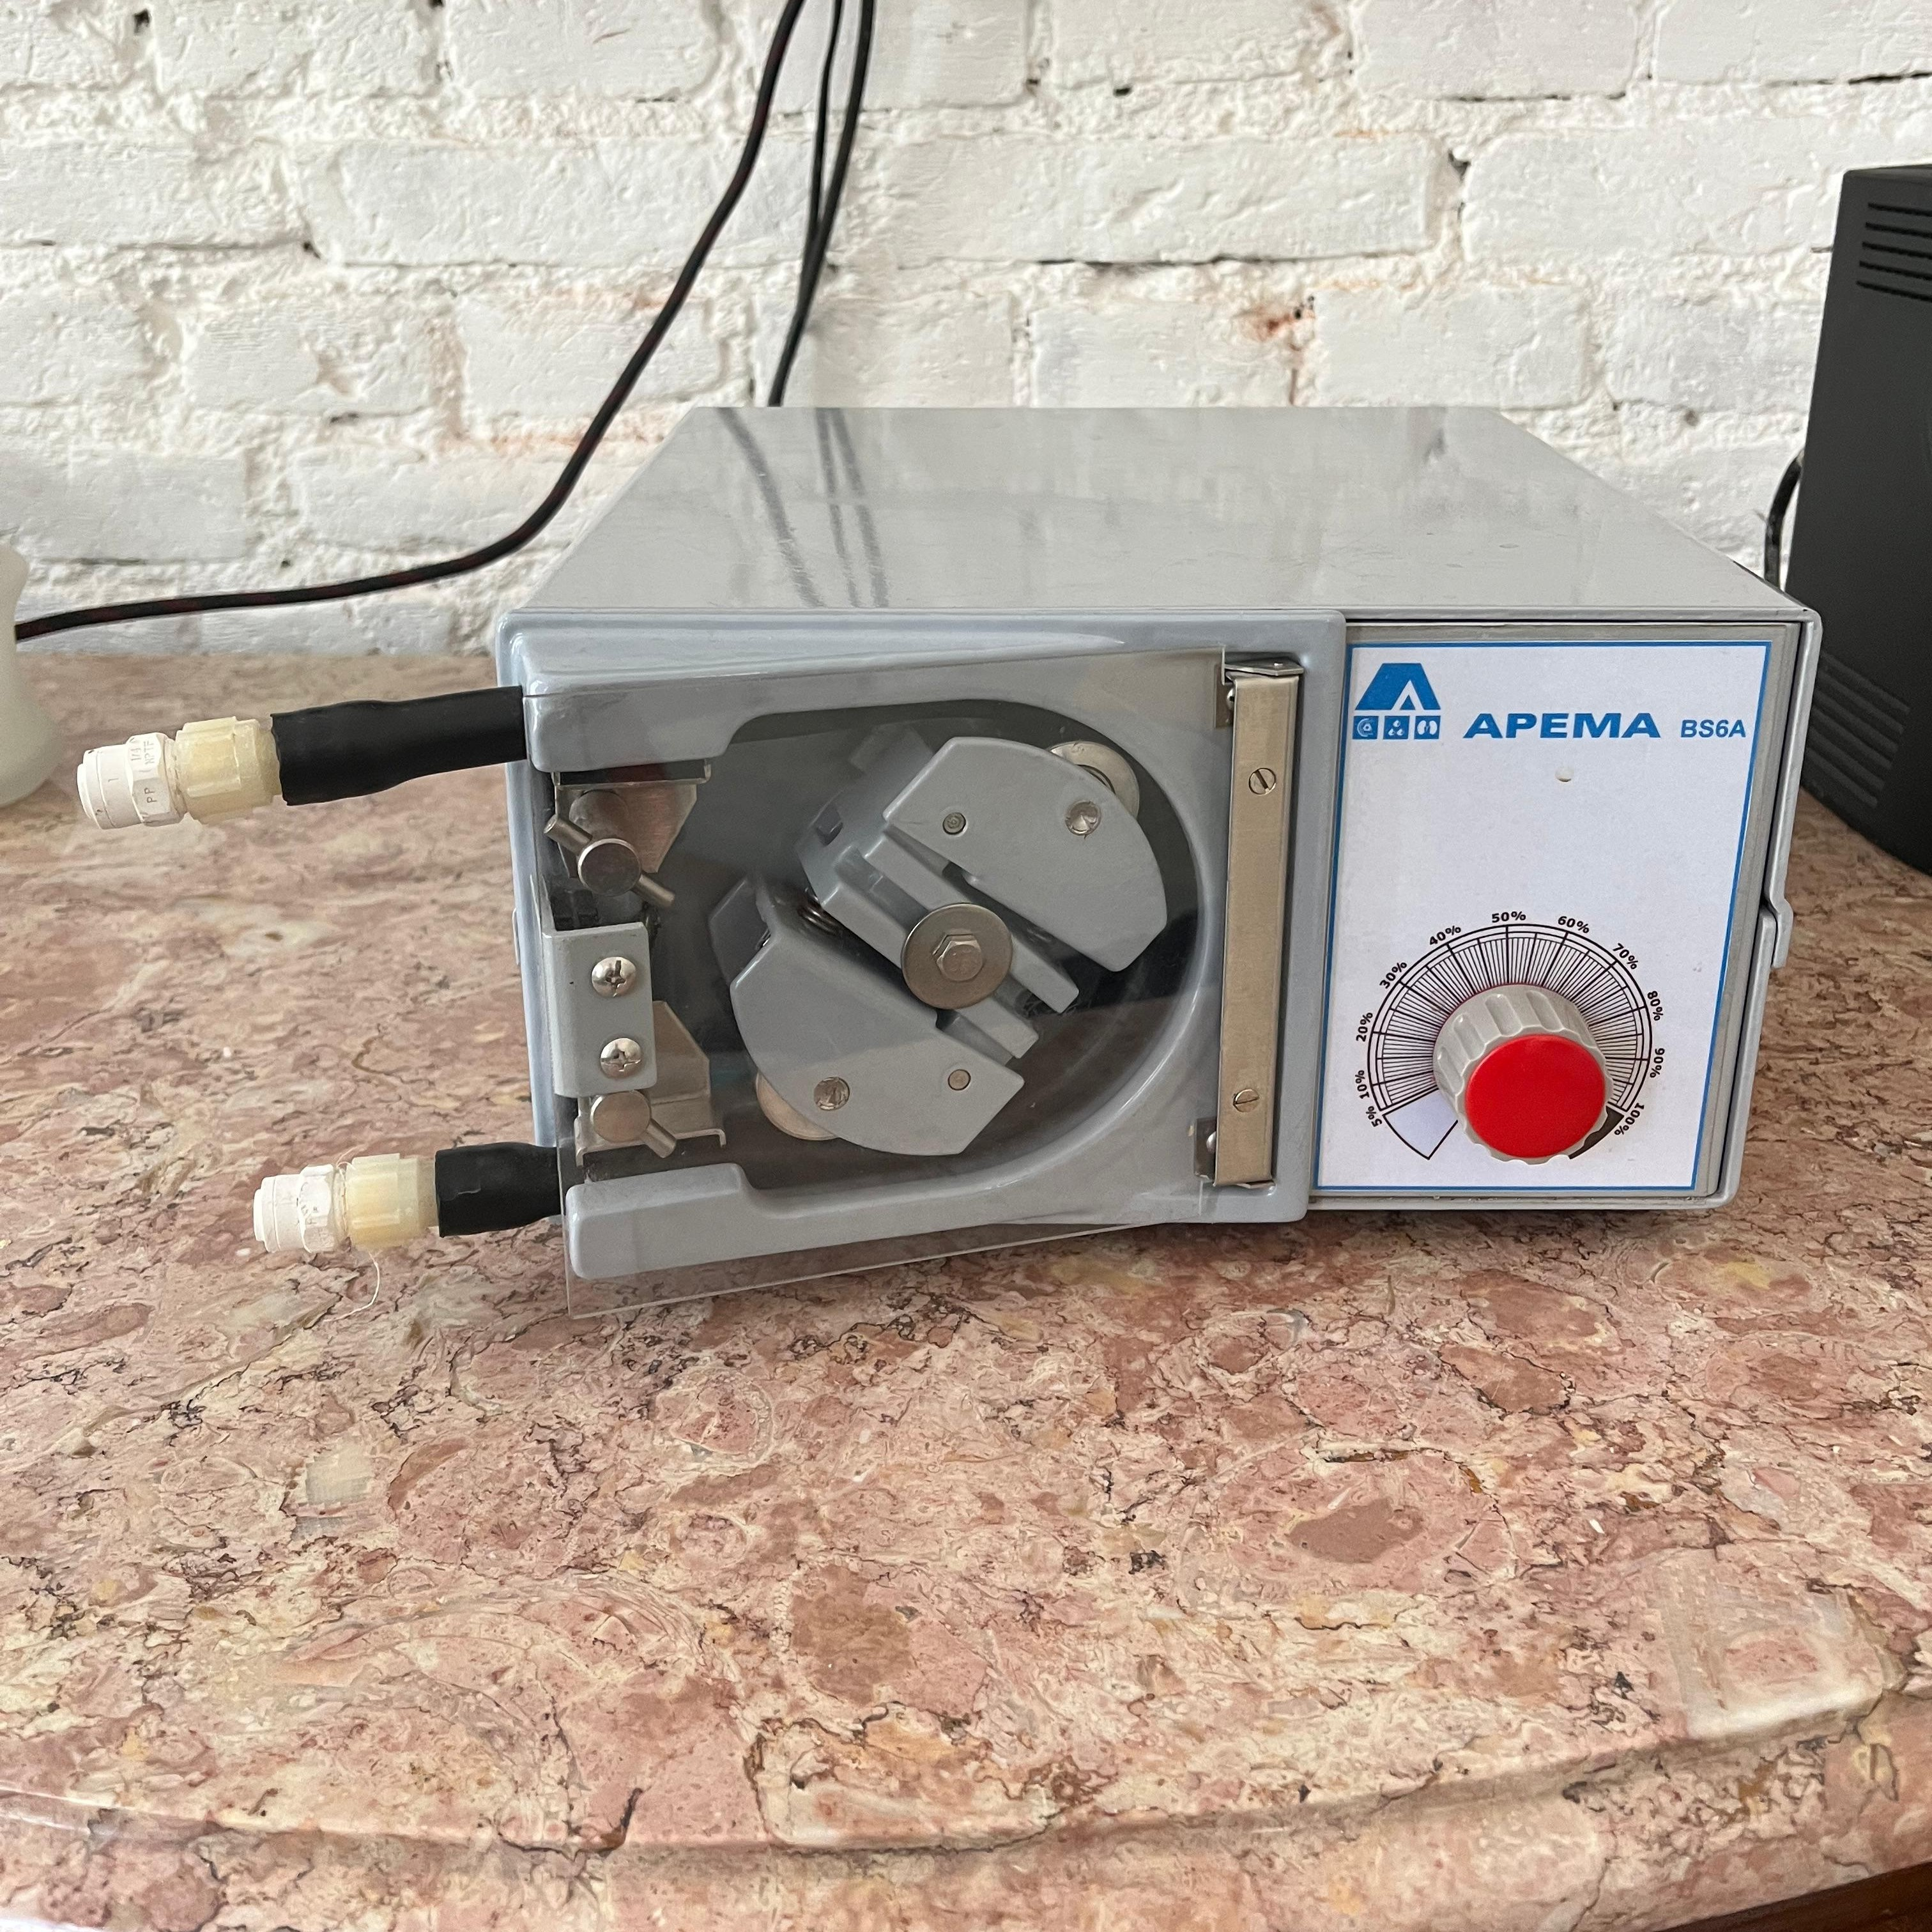
\includegraphics[width=\linewidth, height=7cm]{figures/ch4/APEMA BS6A.jpg}
        \caption{APEMA BS6A device}
        \label{fig:fourth}
    \end{subfigure}

    \caption{Suspended load field trip}
    \label{fig:suspended sediment}
\end{figure}



% In theory, since it was done at different levels of the river, it could potentially indicate a change in concentration from one point upper at Ibicuy to Brazo Largo in the southern, lower part of the study area. From this data, the group could draw even further conclusions.

\subsubsection{Bed load}
Moreover, the bed load was a necessary measurement for our analysis. The method used for this parameter is scraping the bottom layer of the channel with a metal shaped container. The goal is to retrieve samples that represent the granulometry of the bed at different depths. 
The strategy for this measurement is tying a rope to the metal container, dropping it until it reaches the maximum depth of the location. Then, with help of the current or the boat, the person who holds the rope drags the container along with the horizontal movement which gradually collects sediment from the surface. Once this is done, the rope and the container are pulled up and restored in the boat. The last step is to collect some sediment and put it in a plastic bag.  Later on, the captured sediment was sent to the lab where the soil was dried out to find the components, quality and other parameters of the soil such as porosity which would add up to our results. The metal container, as well as the extracts of the sediment samples in the oven are shown in Figure \ref{fig:bed load}. 

\begin{figure}[H]
    \centering
    % First row of subfigures
    \begin{subfigure}[b]{0.6\textwidth}
        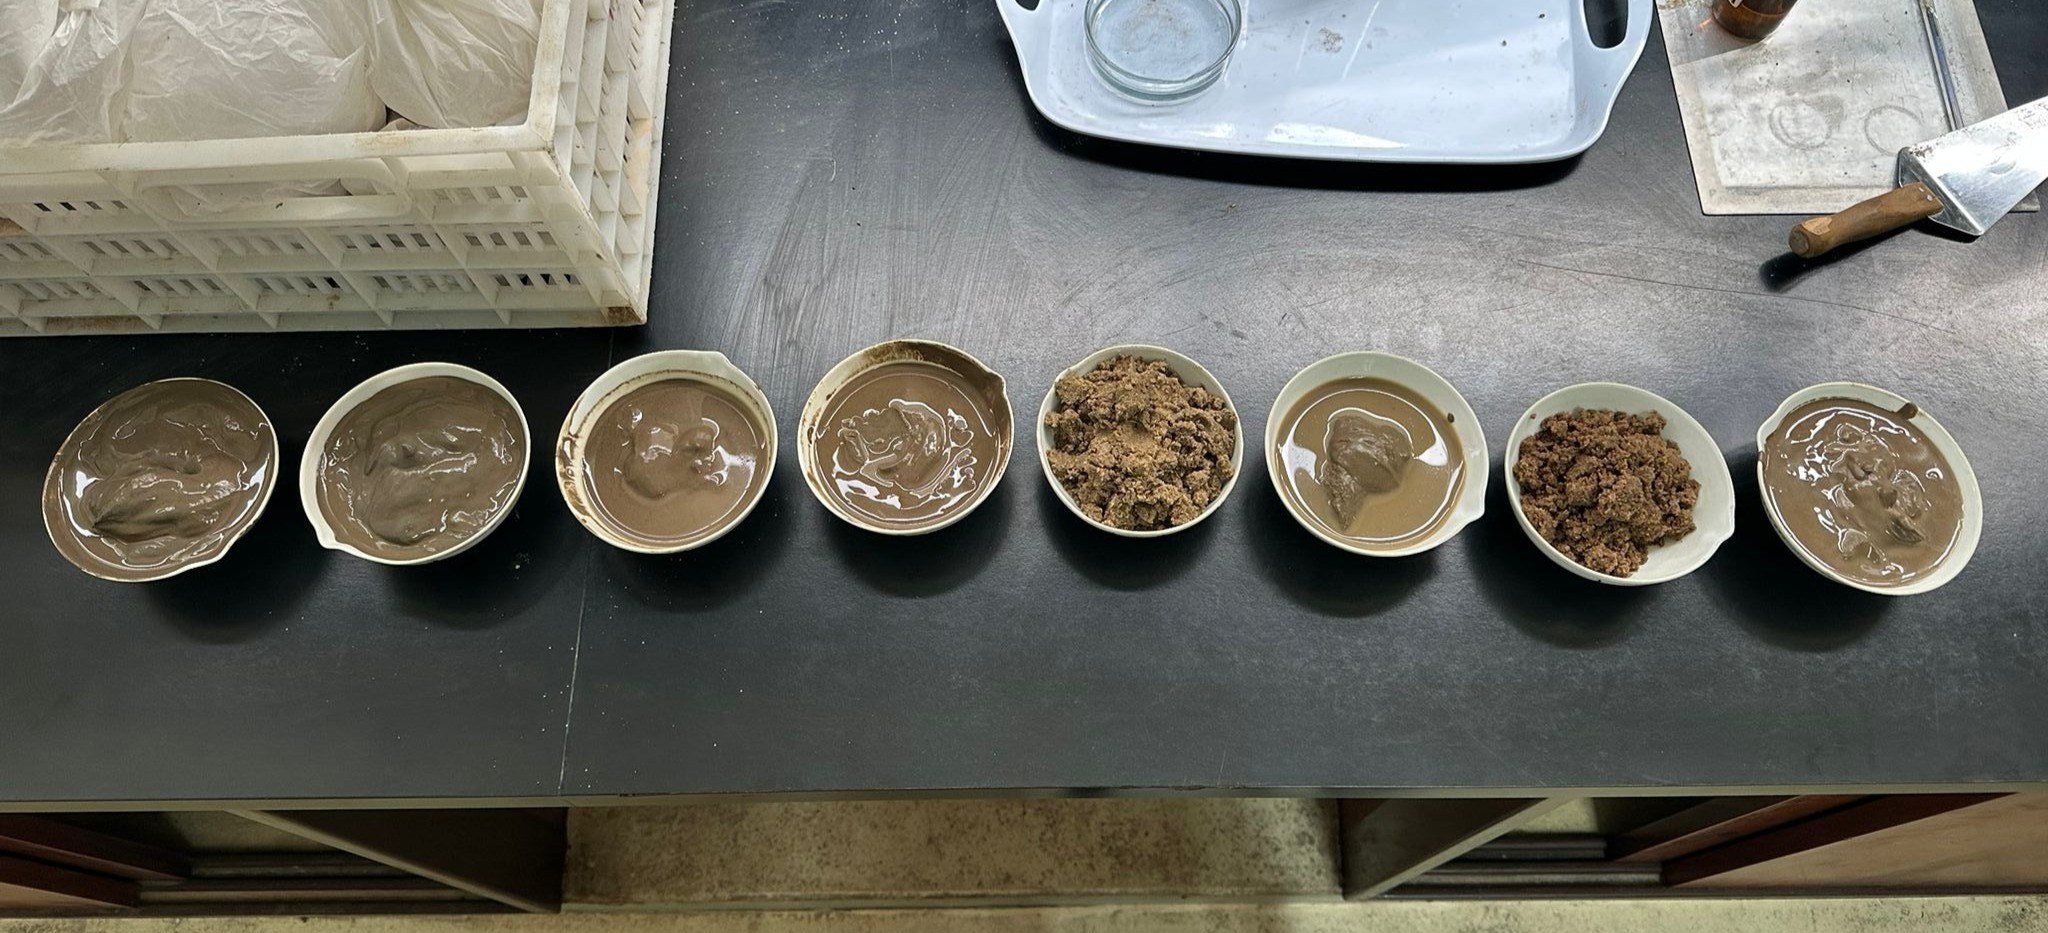
\includegraphics[width= 10cm, height =5cm]{figures/appendixE/soilsamples.jpg}
        \caption{Bed Load Samples from the Fieldwork}
        \label{fig:second}
    \end{subfigure}

    % Second row of subfigures (add some vertical space)
    \vspace{0.5cm}

    % Second row of subfigures
    \begin{subfigure}[b]{0.48\textwidth}
        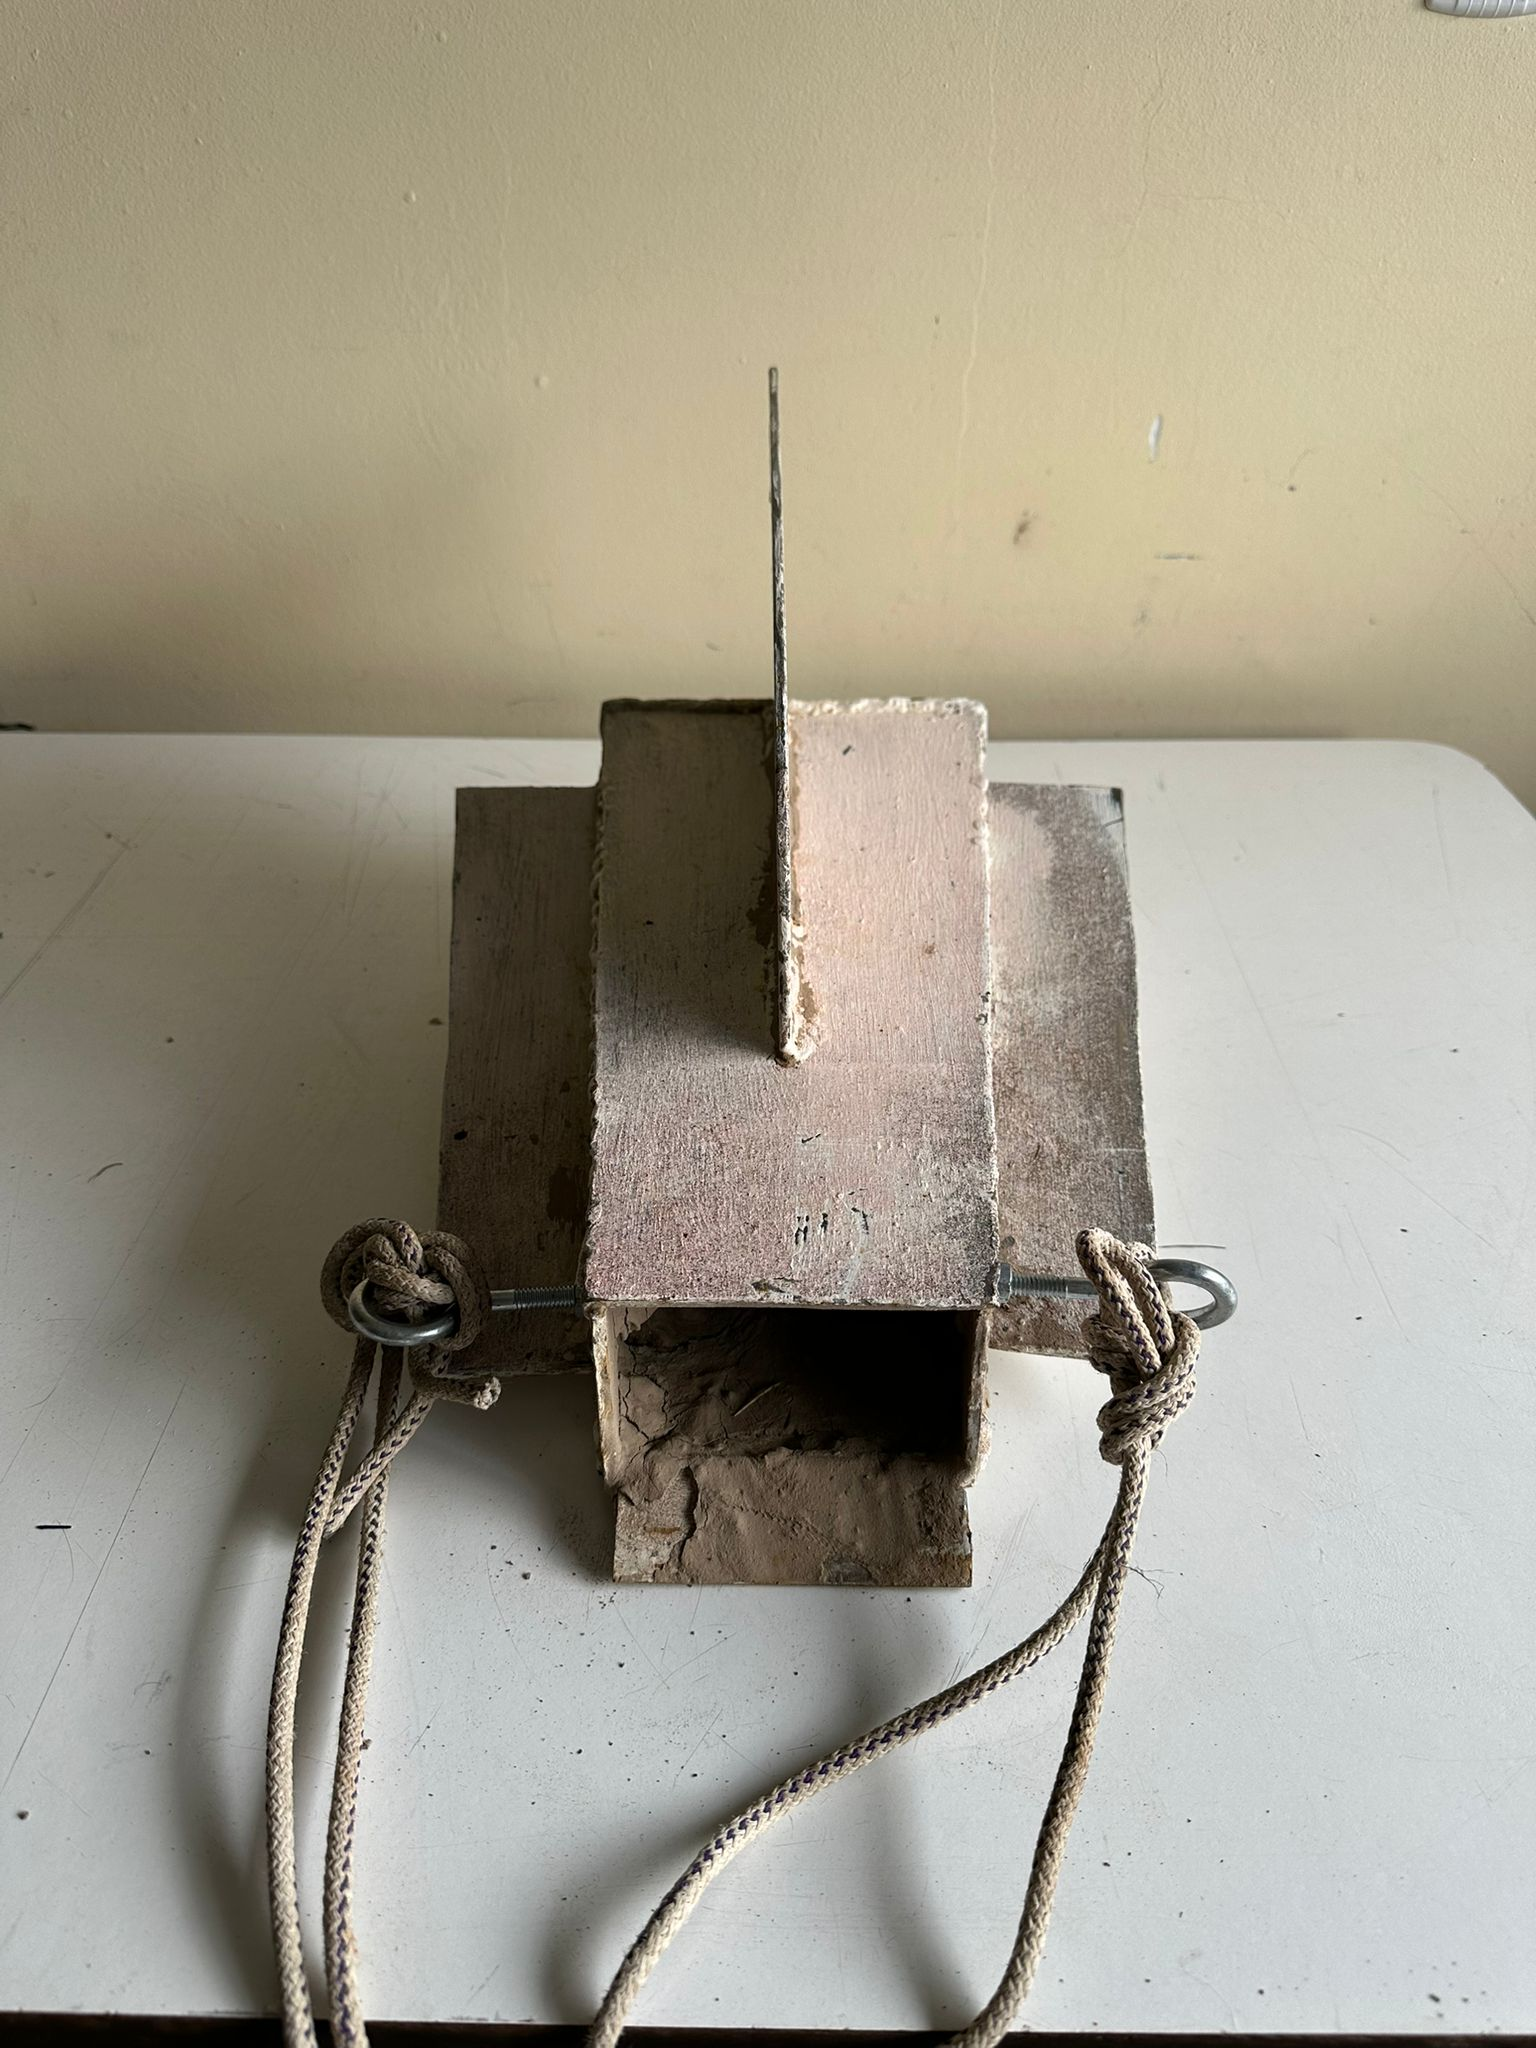
\includegraphics[width=\linewidth, height=7cm]{figures/appendixE/metalcontainer.jpg}
        \caption{Metal Container used}
        \label{fig:third}
    \end{subfigure}
    \hfill
    \begin{subfigure}[b]{0.48\textwidth}
        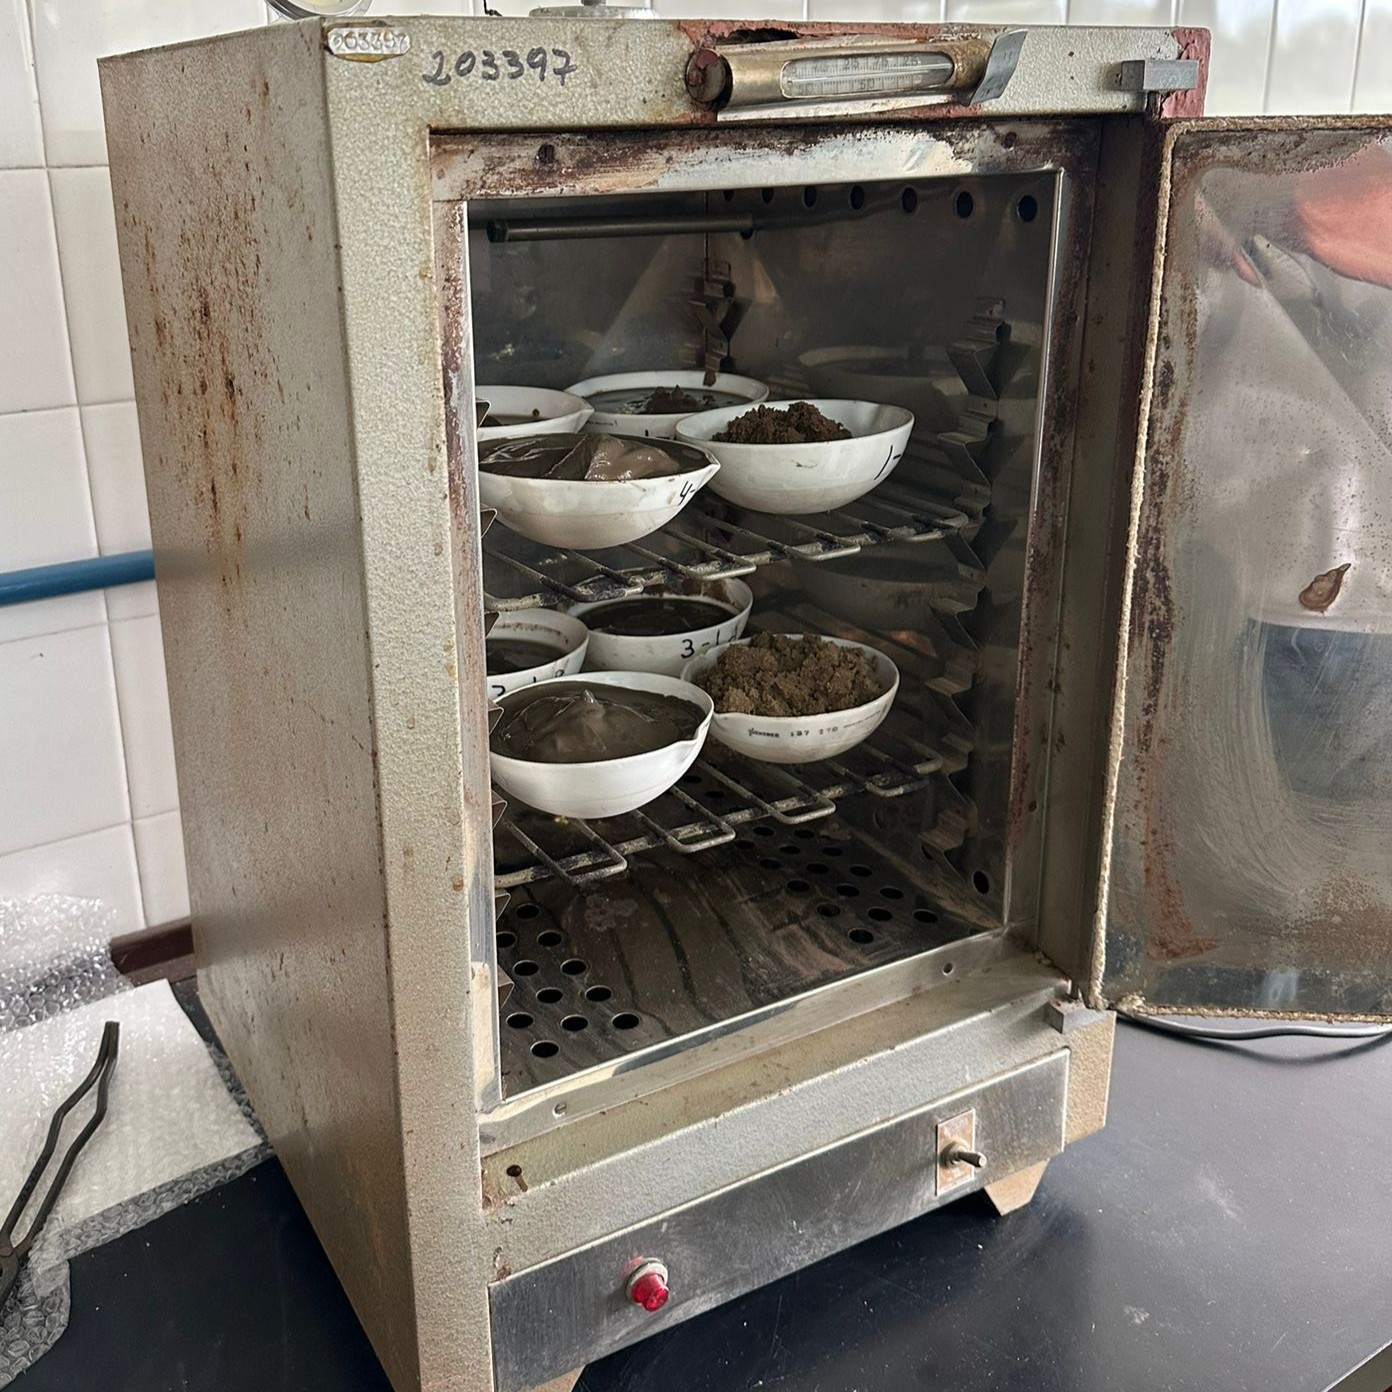
\includegraphics[width=\linewidth, height=7cm]{figures/appendixE/oven.jpg}
        \caption{Oven to dry samples}
        \label{fig:fourth}
    \end{subfigure}

    \caption{Bed Load Measurements}
    \label{fig:bed load}
\end{figure}

The bed load samples were all weighed before they were put in the oven. There are 7 samples collected at 4 different locations. The first three locations are the cross sections around the extracting point in the bifurcation of the Paraná Guazú with the Talabera river. For these three cross sections two samples were taken from the soil, one at 10 meters depth and one at 15 meters depth, approximately. 
The last sample was taken at 10 meters depth in the cross section upstream close to Puerto Ibicuy. The whole collection of the annotated samples can be seen in Appendix \ref{appendix:Lab data}.

\subsubsection{Bathymetry}
To find the bathymetry one can use the ADCP or the Garmin echosounder. 
The bathymetry is the depth of the channel at the position of the boat on a given timestep. Moving over the whole width of the channel yields a longitudinal profile, indicating what depth lies at what coordinates.
The echosounder is attached to a pole on the side of the boat, and dipped into the water while the boat is moving. This pole is connected to the Garmin screen giving the depth and bathymetry of the channel, as seen in the Figure \ref{fig:Garmin}. In addition, this screen allows monitoring of possible bed forms in the river bed. The profile was taken on the whole trajectory between Puerto Guazu to Ibicuy in the morning upstream, and downstream on the end of the afternoon. This profile is seen in Figure \ref{fig:measurements day2}.

\begin{figure}[H]
    \centering
    \begin{subfigure}[b]{0.48\textwidth}
        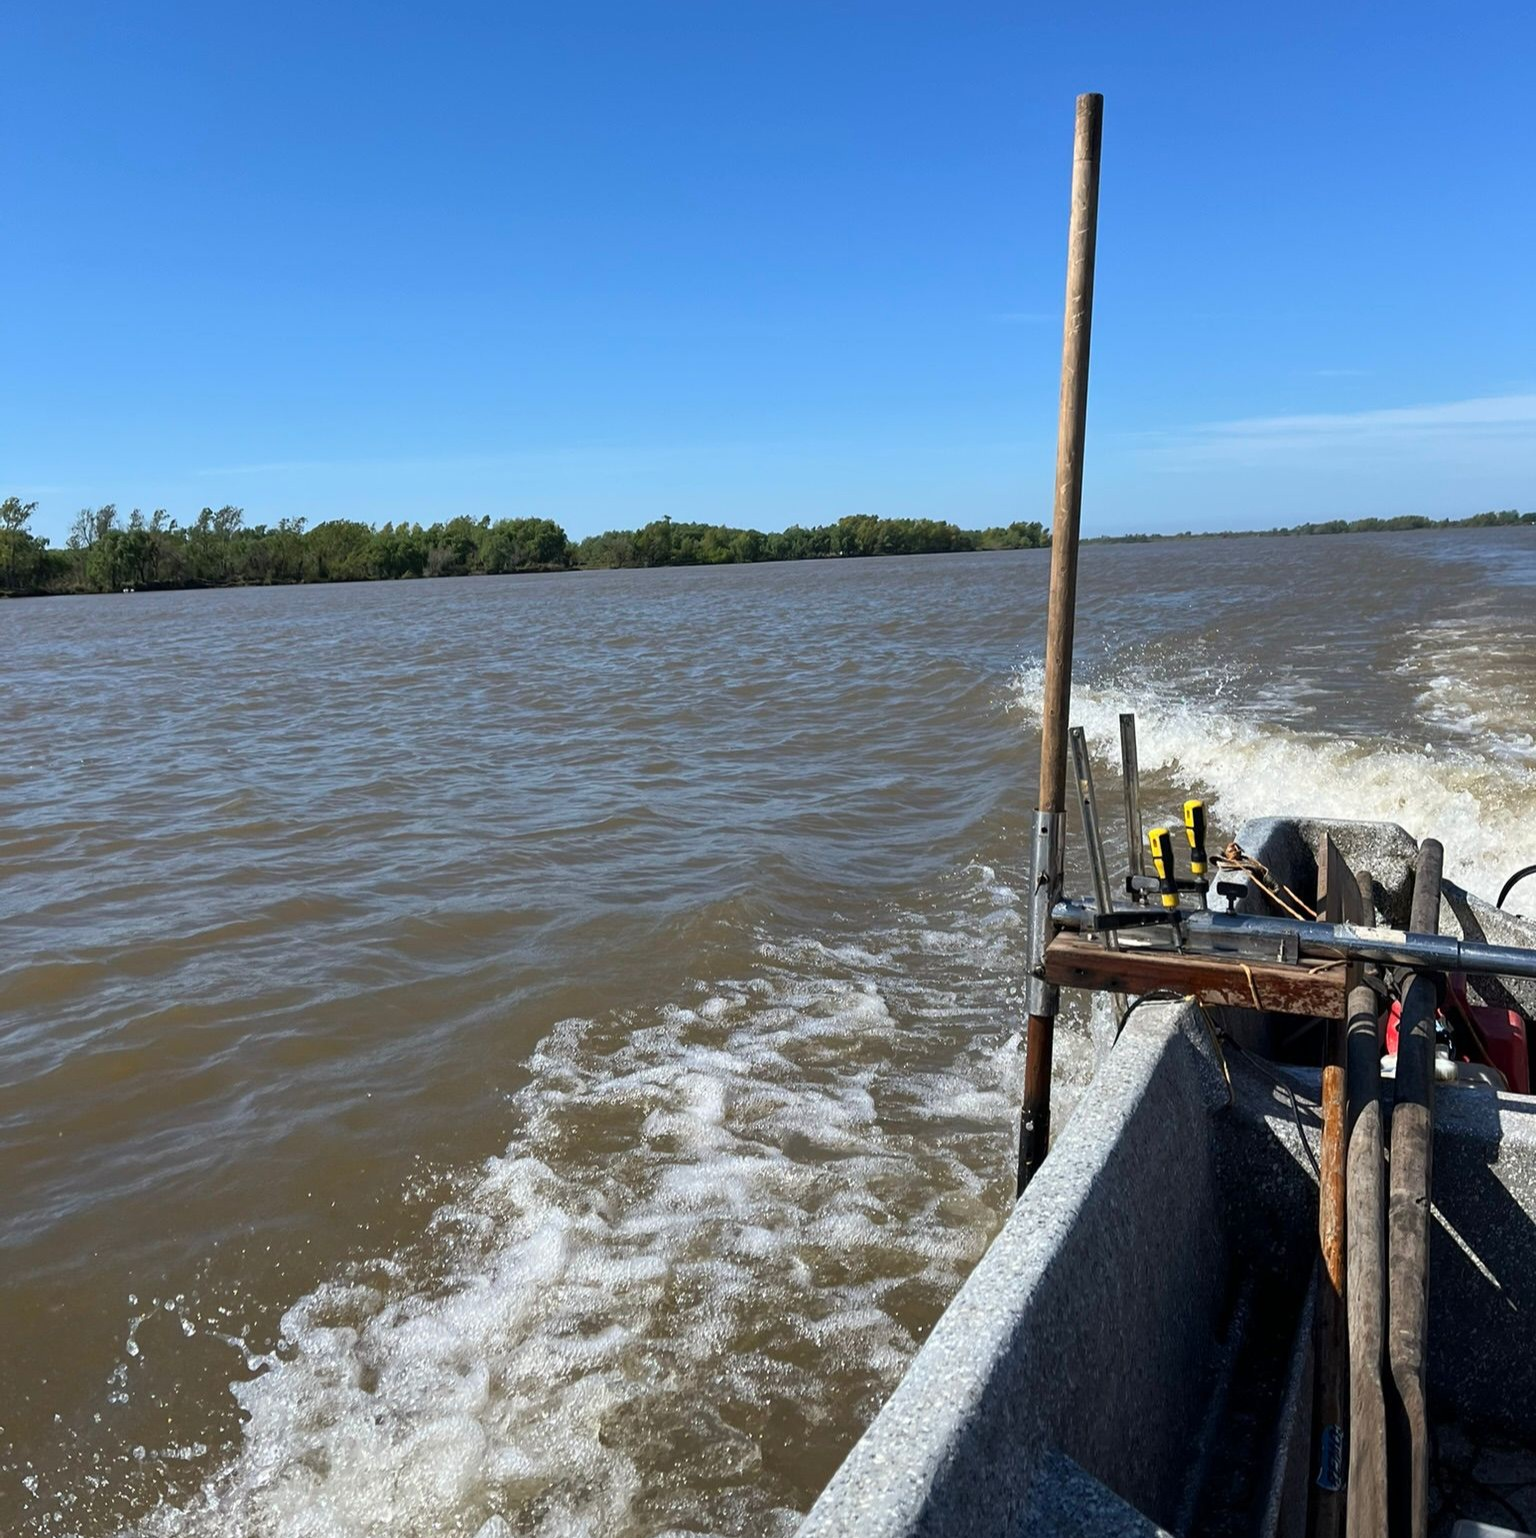
\includegraphics[width=\linewidth, height=7cm]{figures/ch4/Echosounder.jpg}
        \caption{Echosounder attached to boat}
        \label{fig:sontek}
    \end{subfigure}
    \hfill
    \begin{subfigure}[b]{0.48\textwidth}
        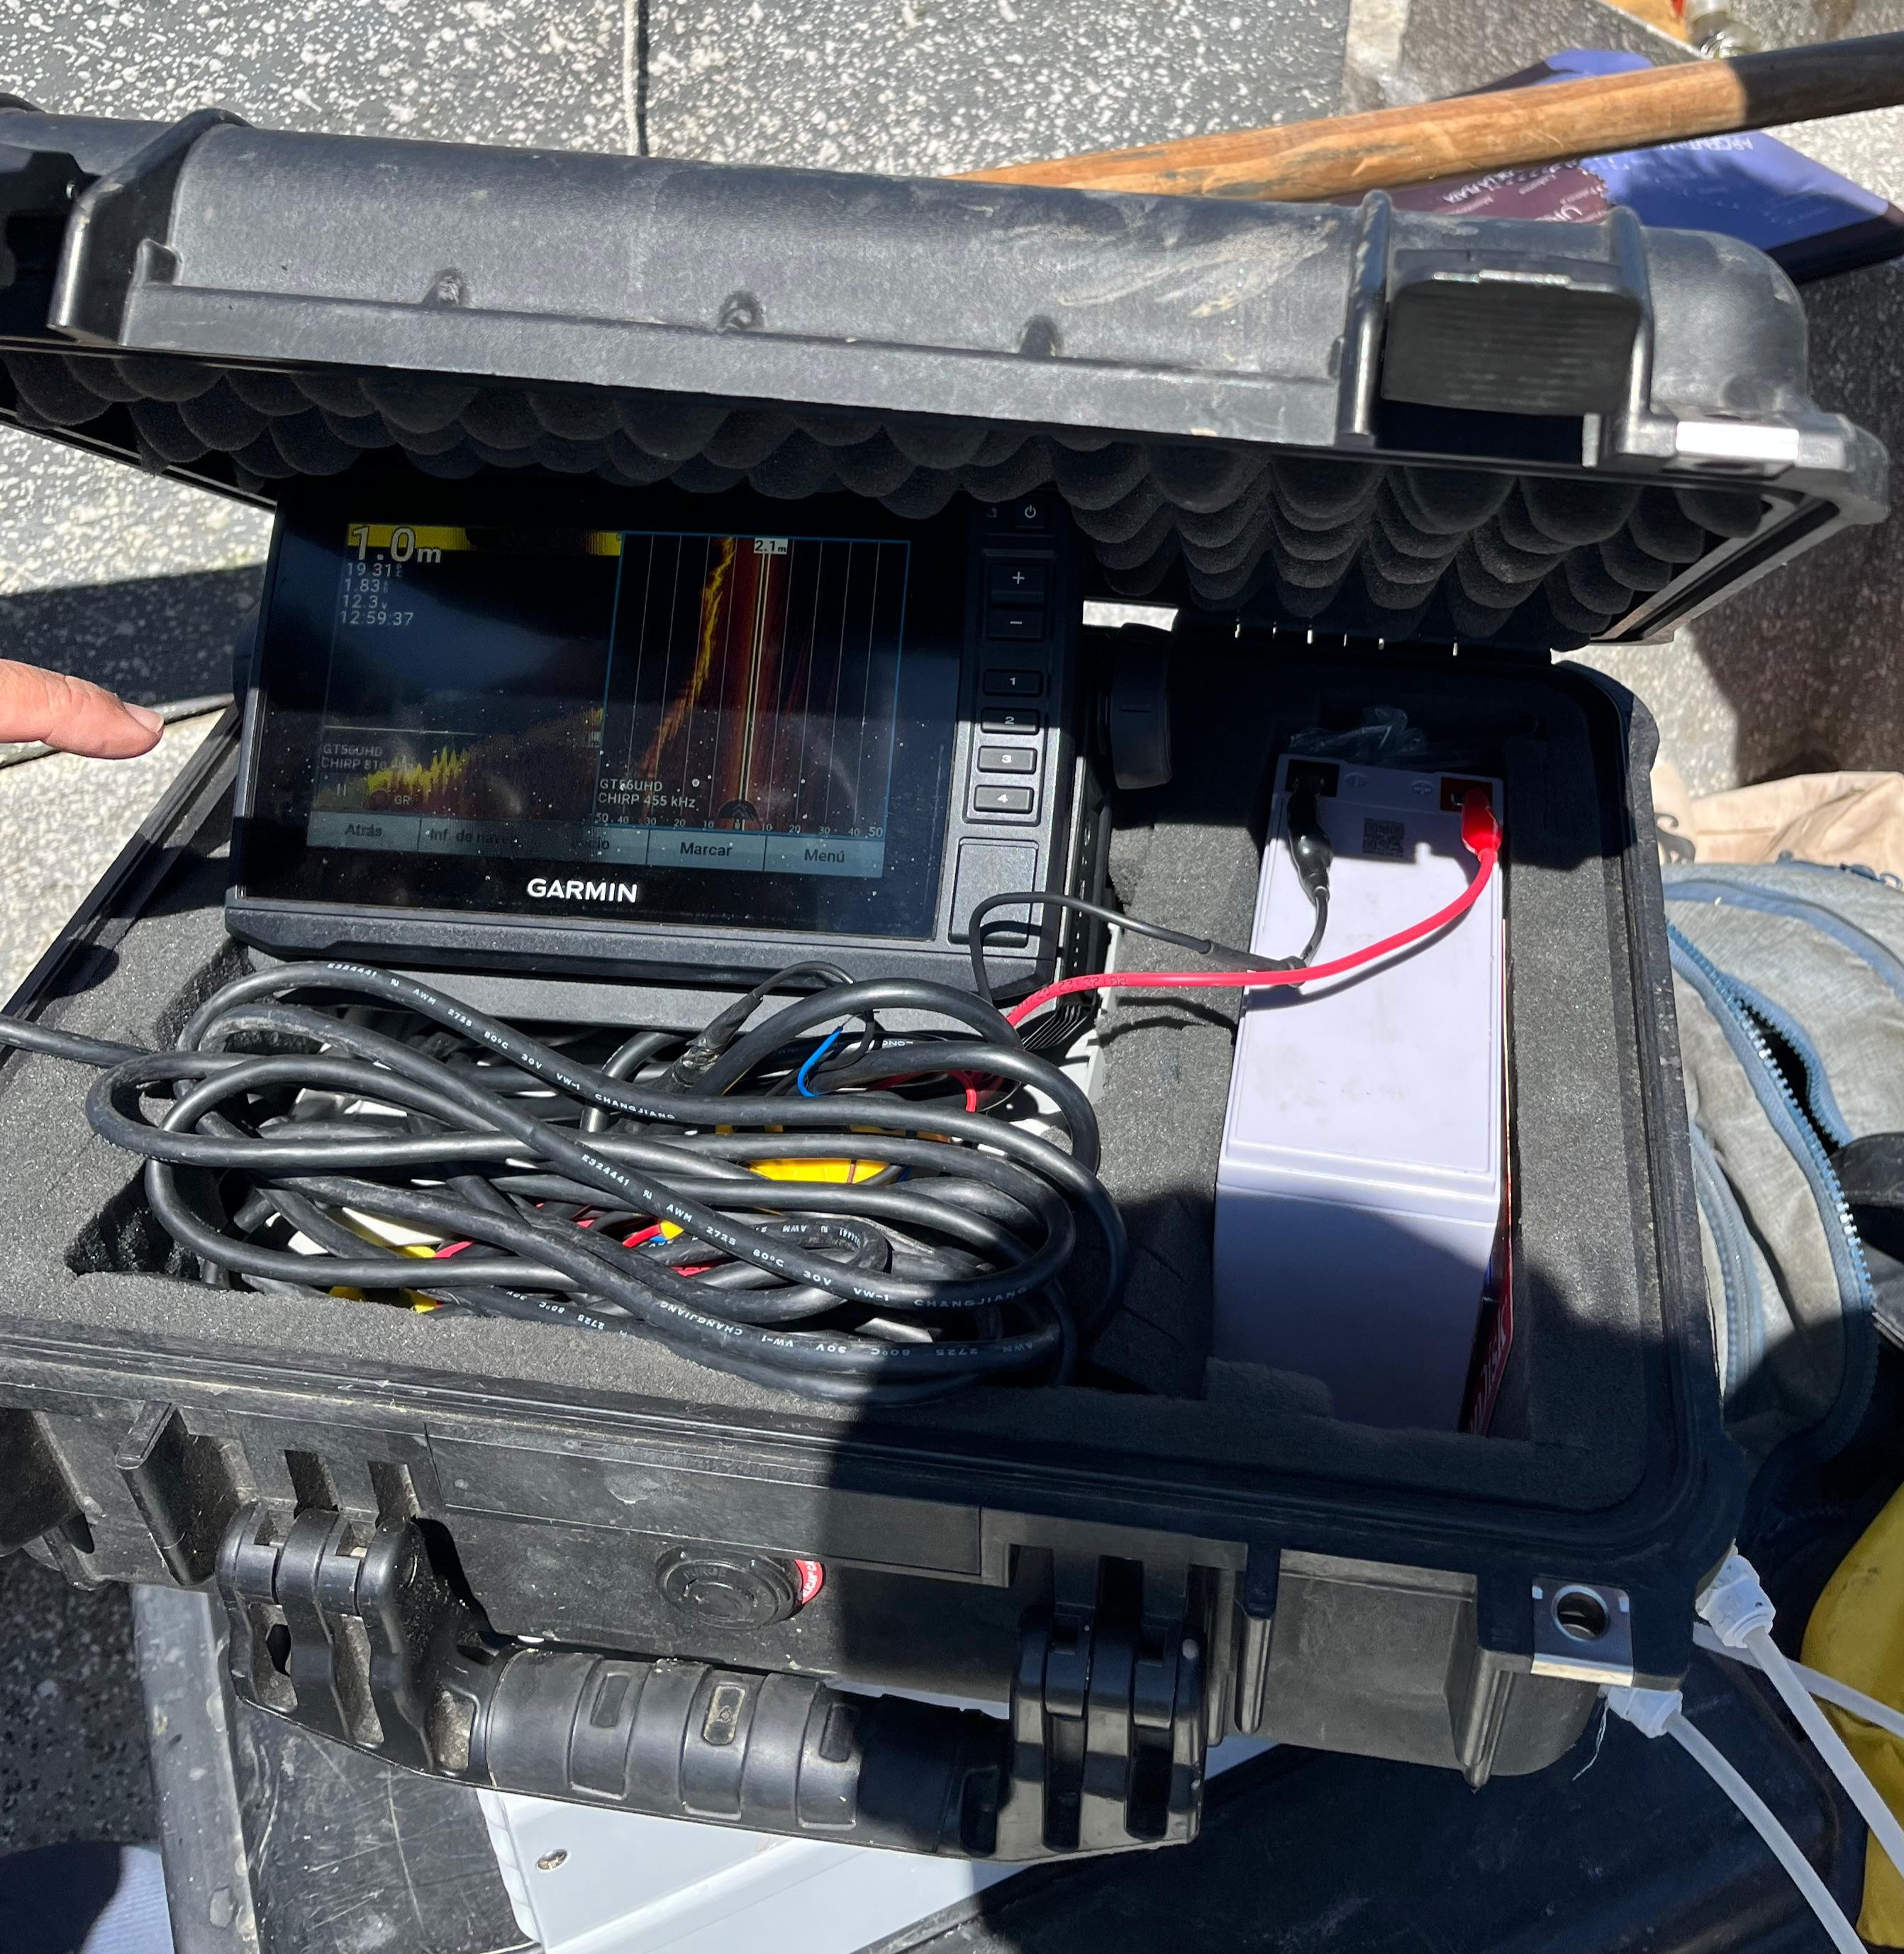
\includegraphics[width=\linewidth, height=7cm]{figures/ch4/garmin.jpg}
        \caption{Garmin material}
        \label{fig:sontek}
    \end{subfigure}
    \caption{Echosounder and Garmin measurements}
    \label{fig:Garmin}
\end{figure}




\subsection{Locations of measurements}
The measurement campaign was divided into two days. The first day, a number of cross sections and sediment samples were recorded at the confluence of the Talabera and the Paraná Guazú. Figure \ref{fig:measurements day1} shows a summary of the performed measurements. In total, three sections were studied with the following measurements per cross section:
\begin{itemize}
    \item 2 ADCP profiles, yielding bathymetry, discharge and flow velocity
    \item 2 bed load samples at different locations with different depths
    \item 5 suspended sediment samples at a single location with varying depths
\end{itemize}

\begin{figure}[H]
    \centering
    \includegraphics[width=0.75\linewidth]{figures/ch4/day1.png}
    \caption{Measurement locations Day 1}
    \label{fig:measurements day1}
\end{figure}

The second day, the research area was expanded by going to Puerto Ibicuy. There, some cross sections were measured in the vicinity of the confluence of the Ibicuy and the Paraná Guazú. In addition, the echosounder was active all day long. Its recorded tracks can be found in Figure \ref{fig:measurements day2}. The following results have been found on day 2:
\begin{itemize}
    \item 6 ADCP profiles. 2 profiles each for the most upstream and most downstream cross section, respectively. 1 profile for those in between. 
    \item 1 bed load sample near Puerto Ibicuy
    \item 2 longitudinal profiles along the confluence of Talabera and Paraná Guazú, measured at the beginning and end of the day to study dune migration
\end{itemize}

\begin{figure}[H]
    \centering
    \includegraphics[width=0.75\linewidth]{figures/ch4/day2.png}
    \caption{Measurement locations Day 2}
    \label{fig:measurements day2}
\end{figure}



\section{Setting up the Sediment Balance}
Using the flow velocity we can derive the concentration of the sediment in the study area. This can be done for several locations in order to get an idea of the quantities of sediment that come in through the Rio Ibicuy. Then the last critical point will help us determine the continuation of the concentration of the sediment in the Rio Parana so that any inconsistencies can be linked with the amount of extracted sand in the intersection of the Parana Guazu and Rio Talabera (in the middle of the three critical points on the right hand side of Figure 4.2).

A mathematical expression/derivation will be explained.

\section{Bank Erosion}
Bank erosion is a recurrent topic in this project. From the introduction, background study, the report has illustrated what bank erosion is, how it can be accentuated by sand mining in the river, and also how it can suck up the land on the riverside. 
In this section, the methodology will be explained as to how one has studied this matter, and how the data was found to get to conclusions.

During the field trip it was noticed through the interviews that a significant amount of people living along the riverside were affected by bank erosion \ref{chap:interviews}. The group took some pictures from the actual conditions in 2025, so that a comparison could be established once older data was obtained. From what we saw, the land was highly eroded, some trees were on the verge of being in the water, while others were already sucked up by the river. This can be seen in the Figures \ref{bankerosion} below taken during the field trip.

\begin{figure}[H]
    \centering
    \begin{subfigure}[b]{0.6\textwidth}
        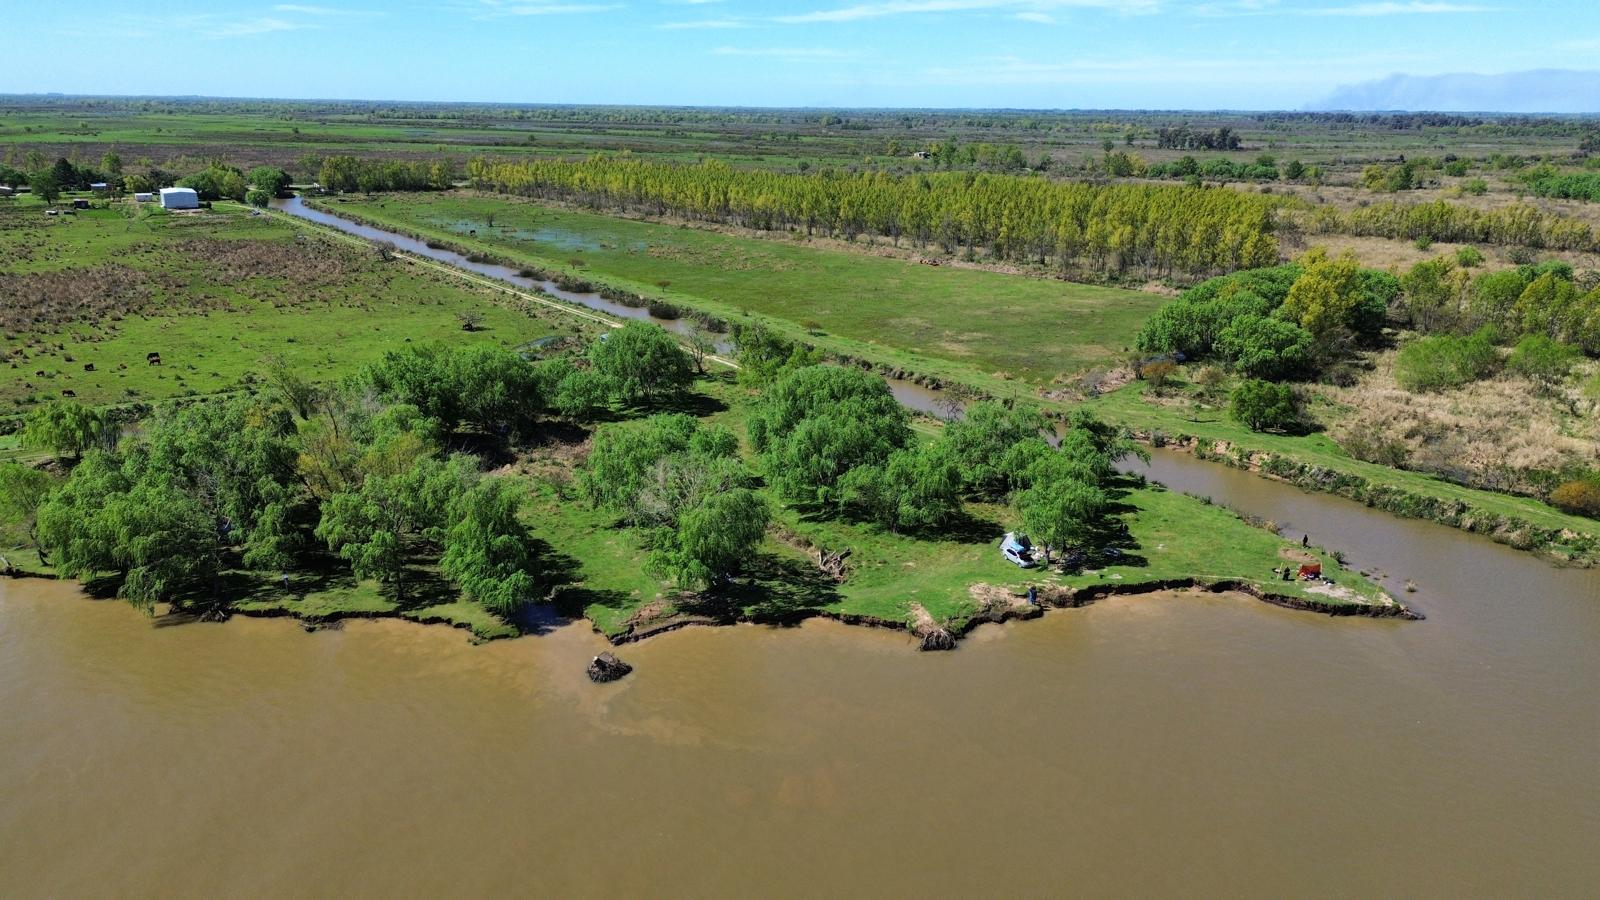
\includegraphics[width=\linewidth, height=6cm]{figures/ch4/bankerosioncamping.jpg}
        \caption{Bank Erosion La Blanqueada}
        \label{fig:sontek}
    \end{subfigure}
    
    \vspace{0.5cm}
    

    \begin{subfigure}[b]{0.6\textwidth}
        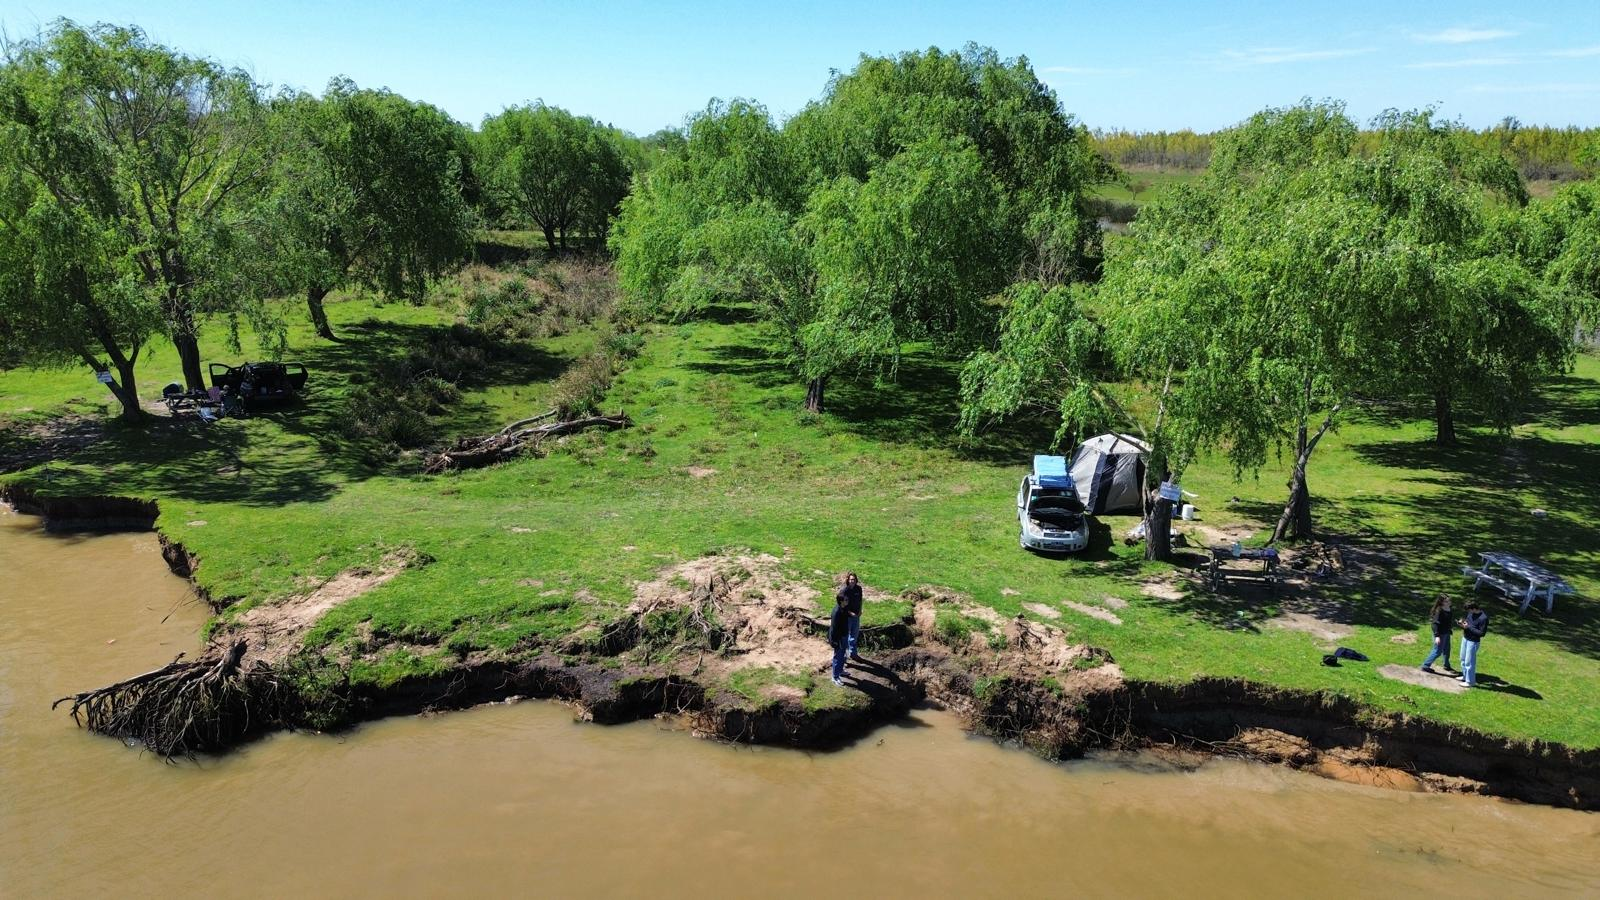
\includegraphics[width=\linewidth, height=6cm]{figures/ch4/bankerosioncamping2.jpg}
        \caption{Bank Erosion Closeup}
        \label{fig:sontek}
    \end{subfigure}
    \caption{Bank Erosion Shots from Field Work}
    \label{fig:Bank Erosion shots from field work}
\end{figure}
\label{bankerosion}


The initial guess from the stakeholders was that the land was eroded up to 30 meters every year which to us; sounded like an impossible number.

Once the fieldwork passed, the comparative study on erosion could begin.

The study started with the Aqua monitor Github code from Deltares which provides an illustrative map of water gains and losses over time. This gave some first insights into the matter.

The satellite database of Deltares was used in Google Earth Engine for different time stamps, starting from 1984. The reason behind this is that the Deltares Aqua Monitor is a tool using Google Earth Engine, containing satellite imagery from 1984 until today. 
 
The choice was made to analyze the data in time batches of 10 years from 1985 until 2005, then in 5 years from 2005 to 2015, and lastly every 2.5 years in the last decade.

A preview of the maps can be seen in Figure \ref{Aqua Monitor Water Changes 1985-2025}below, but the final analysis and conclusions are explained in the next chapter \ref{chapter:data analysis}. 

\begin{figure}[H]
    \centering
    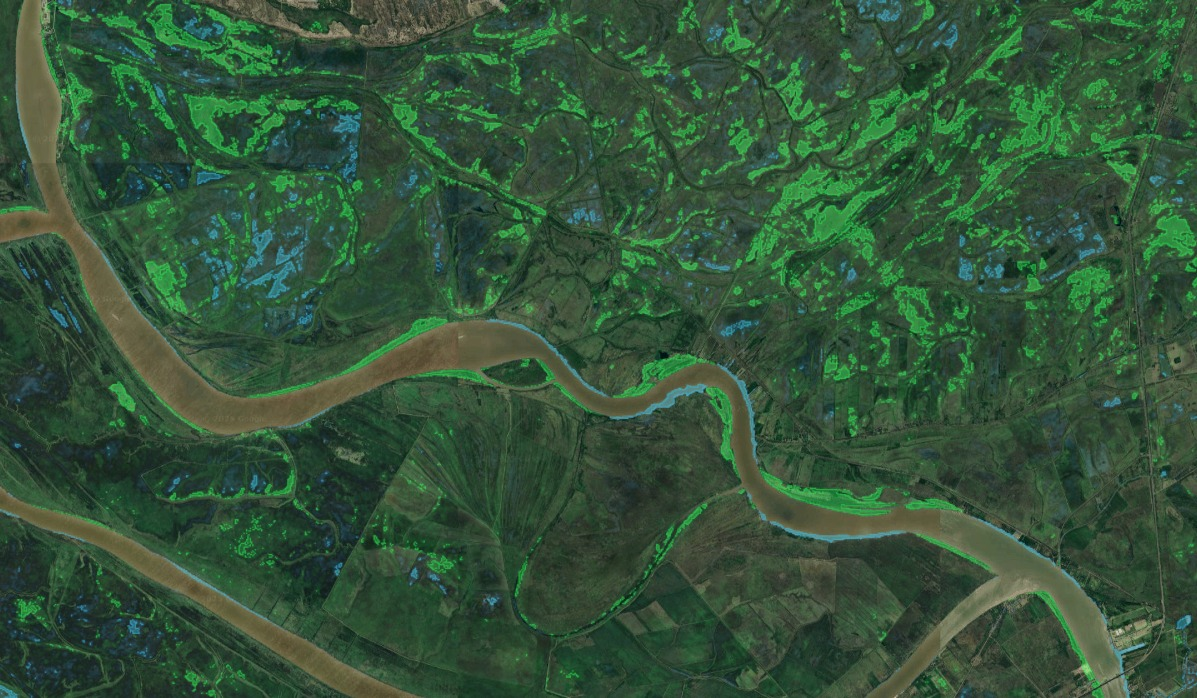
\includegraphics[width=0.75\linewidth]{figures/ch4/1985-2025.jpg}
    \caption{Aqua Monitor Water Changes 1985-2025}
    \label{fig:measurements day2}
\end{figure}
\label{Aqua Monitor Water Changes 1985-2025}

For more clarity, the green parts of Figure \ref{Aqua Monitor Water Changes 1985-2025} are water losses and the blue parts are water gains over time.


For the whole collection of Figures see Appendix \ref{Appendix: Satellite Data}.


\section{Multidisciplinary approach}
The aim of this report is to present a comprehensive assessment of the sustainability of sand mining in the Paraná River. To capture the full scope of the issue, a multidisciplinary approach is adopted. Accordingly, the impacts of sand mining are examined from several perspectives, reflecting the expertise of the authors:

\begin{itemize}
    \item \textbf{Hydraulic}: assessment of the sediment balance and future river flow projections.
    \item \textbf{Geotechnical}: evaluation of risks to riverbank stability and identification of possible mitigation measures.
    \item \textbf{Structural}: analysis of potential effects on infrastructure, along with consideration of structural measures such as quay walls or stone revetments.
\end{itemize}